\chapter{\acrlong{ci}}
\label{ch:sota-ci}

Todo elemento dentro de un entorno se ve influenciado por multitud de variables que determinan en mayor o menor grado su comportamiento. En la mayoría de los casos es muy complicado determinar el grado de efecto de estas variables, identificar las relaciones que existen entre las mismas o incluso determinar cuáles son.

No existe una definición globalmente aceptada de qué es la \acf{ci}. Dependiendo del autor, se la considera desde un sinónimo de la \acf{ai} hasta un campo completamente diferenciado.

En esta tesos hablaremos desde el punto de vista mayoritario, la \ac{ci} como rama de la \ac{ai} que agrupa todas aquellas técnicas que tratan de aprender soluciones a problemas a través del análisis de información presente en conjuntos de datos, en el entorno o ambos.

Por ello, la primera sección del capítulo ofrecerá una visión histórica de la aparición del concepto para justificar el por qué de esta definición. El resto del capítulo introducirá la importancia que tiene el aprendizaje dentro de este área, describirá las técnicas de \acp{ann} y la \acp{fl} necesarias para sentar las bases del posterior desarrollo de la tesis y dará nociones de qué son los agentes y por qué este punto de vista es útil para nosotros.

\section{De \acrlong{ai} a \acrlong{ci}}

Es difícil precisar el comienzo del interés del ser humano por la emular la inteligencia humana. Los silogismos en la antigua grecia para modelar el conocimiento como reglas, los autómatas mecánicos de los filósofos modernos (siglos XVII al XIX) donde los cuerpos vivos son como un reloj o la electricidad (siglos XIX y XX), capaz de animar constructos son sólo ejemplos de cómo cada nuevo avance en la ciencia ha ido acompañado de un intento de simular el cuerpo y mente humanos.

Podemos aventurarnos a decir que a principios del siglo XX se comienza a gestar el área de la \gls{ai} con los trabajos relacionados con los principios del \textbf{conexionismo}\sidenote{
	El enfoque del \textbf{conexionismo} postula que tanto la \textit{mente} como el \textit{conocimiento} son comportamientos complejos que emergen de redes formadas por unidades sencillas (i.e. neuronas) interconectadas. Se puede considerar a Santiago Ramón y Cajal como principal precursor de esta idea por sus trabajos acerca de la estructura de las neuronas y sus conexiónes (e.g. \cite{y1888estructura} y~\cite{ramon1904textura}).
}. Estas ideas saltaron al mundo de la computación hacia mediados del siglo XX, cuando Warren S. McCulloch y Walter Pitts publicaron su trabajo \textit{\enquote{A logical calculus of the ideas immanent in nervous activity}}~\cite{McCulloch1943}\sidenote{Muchos autores prefieren nombrar este hito, junto con el trabajo \textit{\enquote{The organization of behavior}}\cite{hebb19680} de Donald O. Hebb como el punto de partida del área debido a su connotación computacional}, donde se describe el primer modelo artificial de una neurona.

El trabajo suscitó tanta expectación que se comenzó a especular sobre la posibilidad de emular (una vez más) la inteligencia humana en máquinas. Uno de los resultados fue la publicación de un artículo por parte de Alan Turing que comenzaba con la frase \textit{\enquote{Can machines think?}}~\cite{turing1950computing}, introduciendo el famoso Test de Turing\sidenote{
	El \textbf{Test de Turing} es una metodología para probar si una máquina es capaz de exhibir comportamiento inteligente \textit{similar} al del ser humano. En ella, dos humanos ($H_1$ y $H_2$) y una máquina ($M$) están separados entre sí pero pudiendo intercambiarse mensajes de texto. $H_2$ envía preguntas a $H_1$ y $M$ y éstos le responden. Si $H_2$ no es capaz de identificar qué participante es la máquina, se puede concluir que ésta es inteligente.
} por el que el autor pretendía establecer una metodología para determinar si una máquina podía ser considerada inteligente y por tanto podría llegar a pensar\sidenote{
	El concepto de \enquote{pensar} es un tema controvertido incluso en el propio ser humano: ¿es inherentemente biológico? ¿surge de la mente? Tanto si sí como si no, ¿de qué forma lo hace? Por ello existen detractores de la validez del Test de Turing. Un ejemplo es el experimento de la habitación china (Figura~\ref{fig:chinese-room}), donde se demuestra la invalidez argumentando que la máquina ha aprendido a realizar acciones sin \textit{entender} lo que hace y por qué lo hace. Sin embargo, ¿qué garantías tenemos de que el humano sí es capaz? Si los ordenadores operan sobre símbolos sin comprender el verdadero contenido de éstos, ¿hasta qué punto los humanos lo hacen de forma diferente?.
}.

Pocos años después de la publicación del artículo, en el año 1956, se celebró la \textbf{Conferencia Dartmouth}~\cite{mccarthy1956dartmouth}. En ésta, el tema de la conferencia fue la pregunta del artículo de Turing, y el área nació con entidad propia tras acuñarlo John McCarthy como \acrlong{ai}.

A partir de este momento, la investigación en el área recibió mucha atención por parte de investigadores y gobiernos. Después de todo era un área nueva, muy prometedora y con mucho trabajo por delante. Tras su nacimiento el campo comenzó a dar resultados, pero la expectación y las promesas no permitían ver que los resultados se obtenían en problemas relativamente simples, muy formales y en general estériles, donde en realidad no era necesaria demasiada información para generar un conociminto del entorno en el que los modelos se movían.

\begin{figure}[t]
	\centering
	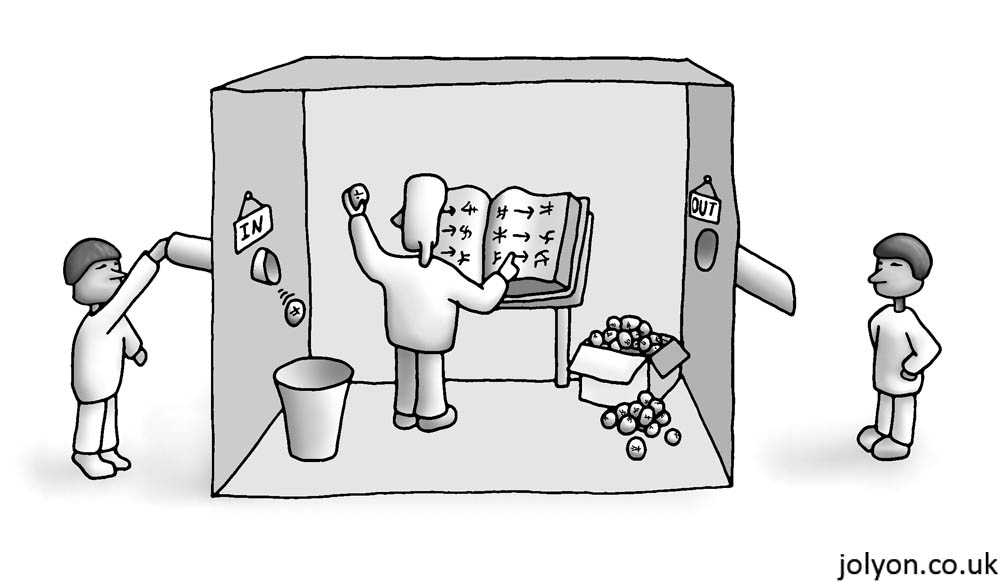
\includegraphics[width=0.72\textwidth]{chinese-room}
	\label{fig:chinese-room}
	\caption[Experimento mental de la \textit{Habitación China}, por John Searle.]{La \textit{Habitación China} de John Searle es un experimento mental por el que se trata de demostrar la invalidez del Test de Turing. Partimeos de un Test de Turing donde la máquina ha aprendido a hablar chino. Reemplazamos la máquina por un humano sin idea de chino pero con un manual de correspondencias de ideogramas. Cuando una persona le manda mensajes en chino, esta otra responde usando el manual, por lo que podemos afirmar que la persona, y por tanto la máquina, no saben chino.}
\end{figure}

Dado que los estudios en el área estaban dominados por aquellos relacionados con las ideas del conexionismo, la publicación del libro \textit{\enquote{Perceptrons}}~\cite{minsky1969perceptrons} de Marvin Minsky y Seymour Papert en 1969 supuso un notable varapalo para las investigaciones. En el se expusieron las limitaciones de los modelos de \acp{ann} desarrollados hasta la fecha, y el impacto fue de tal envergadura que la investigación en el área se abandonó casi por completo. Concretamente el conexionismo prácticamente desapareció de la literatura científica durante dos décadas. Es lo que se conoce como el primer \textit{AI Winter}\sidenote{
	El \textbf{AI Winter} no sólo se produjo por el efecto gurú del libro \textit{Perceptrons}, aunque éste fue la gota que colmó el vaso. A la emoción inicial por los avances le siguieron muchos años de promesas incumplidas, investigación sin resultados significativos, limitaciones de hardware y el aumento de la complejidad del software (los comienzos de la crisis del software \cite{dijkstra1972humble}). Todo ello provocó un desinterés y una disminución de la financiación que se retroalimentaron la una a la otra.
}.

El interés por el campo volvió de nuevo a principios de los $80$ con la aparición en escena de los primeros \glspl{esys}, los cuales se consideran como el primer caso de éxito en la \gls{ai} (\cite{russell2003artificial}). A finales de la década, sin embargo, empezaron a resurgir de nuevo los enfoques conexionistas, debido en gran parte a la aparición de nuevas técnicas de entrenamiento en perceptrones multicapa y por el concepto de activación no lineal en neuronas \cite{rumelhart1985learning, cybenko1989approximation}). En este momento los \acl{esys} empezaron a perder interés frente al nuevo avance del conexionismo\sidenote{
	Esto, evidentemente no sentó bien a los autores prolíficos en \glspl{esys}. Mientras que el enfoque en estos sistemas es el clásico en la computación, donde los problemas (en este caso el conocimiento experto) son resueltos mediante operaciones sobre un lenguaje de símbolos, el enfoque del conexionismo postula que la mente, el comportamiento inteligente, emerge de modelos a más bajo nivel. Por ello, algunas voces se alzaran contra lo que se consideraba el \textit{enfoque incorrecto} de la \gls{ai}. Después de todo, los modelos desarrollados en los métodos clásicos son fáciles de interpretar mientas que los del enfoque conexionista no son del todo deducibles, más aún si estos problemas son de naturaleza estocástica.
}. Esta época se suele identificar como el segundo \textit{AI Winter}, ya que tanto la investigación como las inversiones en el área de \acp{esys} disminuyeron. Sin embargo, el efecto no fue ni mucho menos equiparable al de el primero.

Junto con el resurgir del conexionismo, otras técnica alineadas como la \gls{fl} o los \glspl{ga} también ganaban popularidad, y entre ellas retroalimentaban los exitos gracias a sus sinergias. Esto provocó una explosión de terminologías para diferenciar las investigaciones en curso de la propia \gls{ai} clásica. Por un lado se evitaba el conflicto, nombrando las áreas de trabajo con un término más acorde con el comportamiento o técnica utilizada. Por otro, se separaba de las connotaciones negativas que fue cosechando la \gls{ai} con el paso de los años (i.e. promesas, pero no resultados).

Lo verdaderamente interesante es ver la evolución de la literatura durante estos años. En el nacimiento del campo, se buscan literalmente máquinas que piensen como humanos, o al menos seres racionales, con mente. Con el paso de los años, el área va tendiendo hacia la búsqueda de conductas y comportamientos inteligentes cada vez más específicos. Este hecho se hace más patente en este momento, donde cada investigación se nombra de cualquier forma menos con el término \gls{ai} (e.g \gls{ml}, \gls{rs}, o \gls{nlp}). Es evidente que la \gls{ai} se puede observar desde diferentes puntos de vista, todos perfectamente válidos. En~\cite{russell2003artificial}, tras un análisis de las definiciones existentes en la literatura por parte de diferentes autores, se hace énfasis en este hecho mostrando los diferentes puntos de vista a la hora de hablar de lo que es la \gls{ai}. El resumen se puede observar en la figura~\ref{fig:different-povs-ai}.

Volviendo al tema de la terminología, muchas de las técnicas se fueron agrupando dentro de diferentes áreas. Una de ellas es la conocida como \acrlong{ci}. Dado que persigue el mismo objetivo a largo plazo y que surje de la propia \gls{ai} parece lógico mantenerla como un subconjunto y no como un nuevo campo del conocimiento humano. Sin embargo, algunos autores abogan por que la \gls{ci} es un campo diferenciado de la \gls{ai}.

Podemos definir la \acrlong{ci} como la \enquote{\textit{rama de la \gls{ai} que aporta soluciones a \textbf{tareas específicas} de forma \textbf{inteligente} a partir del aprendizaje mediante el uso de \textbf{datos experimentales}}}. A diferencia de la aproximación clásica de la \gls{ai}, se buscan aproximaciones a las soluciones y no las soluciones exactas. Esto es debido a que muchos problemas son de naturaleza compleja, ya sea por la relación entre sus multiples variables, a la falta de información o a la imposibilidad de traducirlos a lenguaje binario.

\begin{figure}
	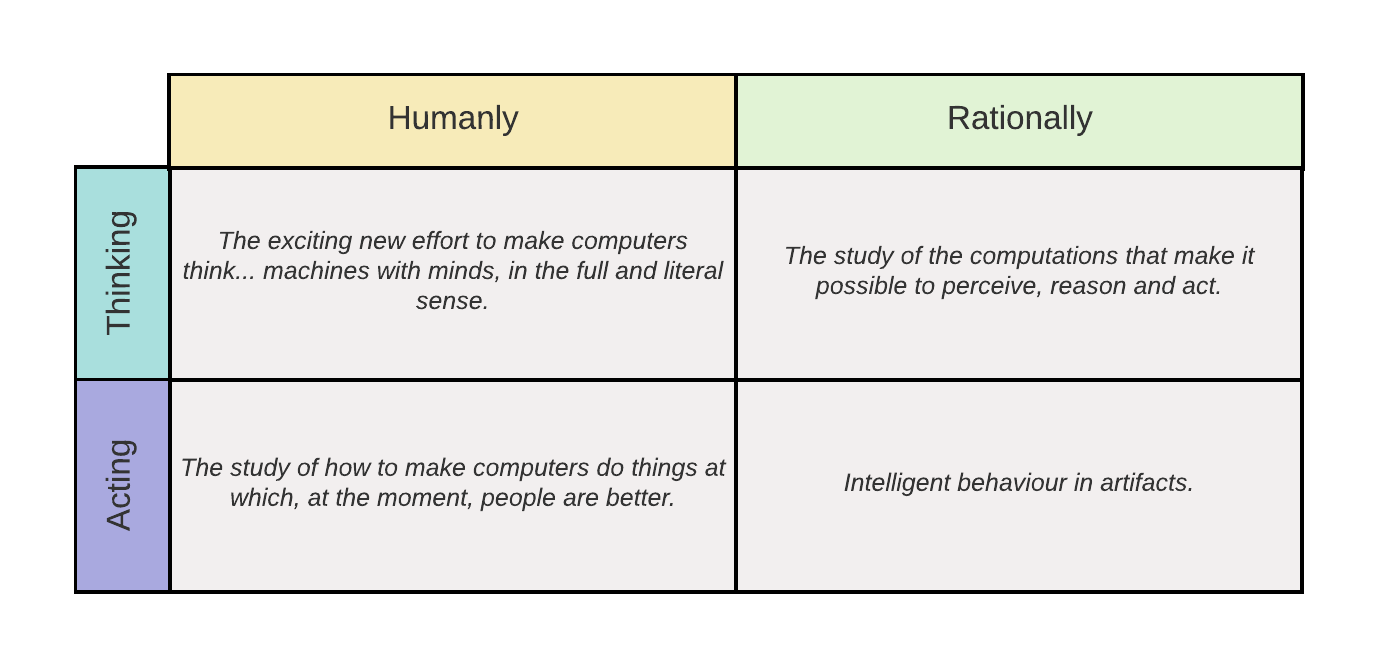
\includegraphics{different-povs-ai}
	\caption[Diferentes objetivos perseguidos por la \acrlong{ai}.]{Diferentes objetivos perseguidos por la~\acrlong{ai}. Las filas diferencian entre pensamiento o comportamiento mientras que las columnas separan entre inteligencia humana o el ideal de la inteligencia (racionalidad). Fuente: \textit{Artificial Intelligence: A Modern Approach ($3^{rd}$ Ed.)},~\cite{russell2003artificial}.}
	\label{fig:different-povs-ai}
\end{figure}

Se puede establecer el año $1994$ como en el que la \acrlong{ci} nace formalmente como área, coincidiendo con el cambio de nombre del \textit{IEEE Neural Networks Council} a \textit{IEEE Computational Intelligence Society}\sidenote{
	\url{http://cis.ieee.org/}
}. Poco antes, en $1993$, Bob Marks presentaba las que él consideraba diferencias fundamentales entre la \acrlong{ai} clásica y la \acrlong{ci}, resumiéndolas en la siguiente frase:

\blockquote{Neural networks, genetic algorithms, fuzzy systems, evolutionary programming, and artificial life are the building blocks of \ac{ci}.}

Durante estos años ganaba popularidad también el concepto del \gls{sc} en contraposición con el \gls{hc}. El \gls{sc} engloba las técnicas que buscan resolver problemas con información incompleta o con ruido. Debido a que el conjunto de técnicas definidas como consituyentes del \gls{sc} son las mismas que se usan en la \gls{ci} algunos autores consideran ambos términos equivalentes. Nosotros consideramos que el \gls{sc} es un punto de vista de la computación a diferencia de la \gls{ci}, la cual es un área de específica dentro de la \gls{ai} hace uso de métodos incluídos en el concepto \gls{sc}.

\marginnote{
	\textbf{\gls{hc} y \gls{sc}} son la forma de referirse a la computación convencional frente al \gls{sc}. El \gls{hc} basa sus técnicas en aquellas basadas en modelos analíticos definidos de forma precisa y que en ocasiones requieren mucho tiempo de cómputo. Están basados en lógica binaria, análisis numérico, algoritmos y respuestas exactas. El \gls{sc} por otro lado es tolerante a la imprecisión y al ruido y tiende a llegar a soluciones aproximadas de manera más rápida. Se basa en modelos aproximados, emergencia de algoritmos y modelos estocásticos.
}

Hoy en día la \gls{ci} es un área con muchas aplicaciones prácticas en una variedad muy distinta de campos de la ciencia y con muchos temas de investigación por explorar. Por ello, esta tesis pretende la exploración de una parte concreta de este área en el tema del modelado de comportamiento humano en el problema de la conducción.

\section{El rol del aprendizaje en la \acrlong{ci}}
\label{s:the-learning-role}

El cambio más notorio entre los dos puntos de vista de la \gls{ai} tradicional y la de la \gls{ci} es el concepto de entrenamiento, es decir, pasar de \textit{\enquote{desarrollar un programa para resolver un problema}} a \textit{\enquote{entrenar un modelo para que aprenda la solución}}. Éste es el concepto de \textbf{aprendizaje}, y al proceso de ajuste del modelo a la solución buscada \textbf{entrenamiento}.

Las técnicas de aprendizaje se clasifican dependiendo de la forma en la que entrenan los modelos. Podemos identificar tres clases principales de técnicas de entrenamiento las cuales se describen a continuación:

\begin{itemize}
	\item \textbf{Aprendizaje supervisado}. Supongamos que disponemos de un modelo denotado por $M_V(V, I) = O$ donde $V$ es el conjunto de variables de determinan el comportamiento de $M_V$ y donde $I$ es un conjunto de valores (características) de entrada para las que el modelo obtiene un conjunto $O$ de valores de salida. Entonces, la forma de entrenar al modelo, es decir el \textit{algoritmo de entrenamiento} se encargaría de, a partir de un conjunto de la forma $D = {(I_i, O_i) | \forall i \in \mathbb{N}}$, donde cada $O_i$ es la salida esperada del modelo a la entrada $I_i$, modificar los valores de las variables del conjunto $V$ para ajustar lo más posible $O_i$ a $O$ dado $I_i$.
	\item \textbf{Aprendizaje no supervisado}. Es el proceso por el cual un modelo aprende a partir de datos en brutos sus relaciones y extrae patrones, sin saber qué son esos datos ni recibir supervisión (a diferencia del aprendizaje supervisado donde los datos incluyen un valore de entrada y su salida correspondiente). En general, los algoritmos pertenecientes a esta categoría se dedican al problema del \textit{clustering}, es decir, identificar grupos de elementos cercanos en el espacio basándose en la suposición de que el comportamiento de dos elementos es más parecido cuanto más cerca están el uno del otro. Algunos ejemplos de técnicas que basan su entrenamiento en un esquema no supervisado son los mapas autoorganizados (SOM), los autoencoders o las redes de creencia profunda (DBN de Deep Belief Network).
	\item \textbf{Aprendizaje por refuerzo}. En este pardigma, el algoritmo ajusta el modelo de acuerdo a políticas de recompensa o penaliación en función de lo bien o lo mal que el modelo está desempeñando la tarea de acuerdo a una métrica determinada. 
\end{itemize}

Algunos autores hacen uso de técnicas pertenecientes a ambos paradigmas en forma de aproximación híbrida para suplir deficiencias u optimizar/acelerar el aprendizaje. Un claro ejemplo lo podemos ver en \cite{Hinton2006}, donde los autores hacen uso de \textit{autoencoders} como técnica no supervisada para la inicialización de los pesos de una red neuronal y posteriormente realizan un entrenamiento supervisado para la optimización es éstos.

Esta tesis se dedica al modelado de comportamiento entrenando a partir de datos reales de conducción, por lo que el discurso se centrará únicamente en el esquema de aprendizaje supervisado. En él, los algoritmos de entrenamiento dependen del modelo a usar (no es lo mismo un algoritmo de entrenamiento para una red neuronal recurrente que para un perceptrón multicapa), y suelen ser usados principalmente para la solución a problemas de \textbf{clasificación} (i.e. determinar si un elemento dada sus características pertenece o no a determinado conjunto) y de \textbf{regresión}, esto es, ajustar las salidas de un modelo para ajustarse lo máximo posible al valor real del sistema modelado.

\subsection{Epochs, conjuntos de entrenamiento, test y validación}

La terminología general que se usa en la \gls{ci} no es demasiado compleja (con la salvedad de los nombres de técnicas y algoritmos). A continuación se resumen los más importantes:

\begin{figure}
	\missingfigure[figheight=4cm]{Ilustración con los distintos conjuntos de datos}
	\caption[Separación clásica de conjuntos de datos en tareas de \acrlong{ml}.]{Los diferentes tipos de conjuntos de datos existentes.}
	\label{fig:different-kinds-of-datasets}
\end{figure}

\paragraph{Conjunto de datos o \textit{dataset}}

Se refiere al conjunto total de ejemplos o datos del que disponemos. Se presupone que el dataset mantiene una distribución de datos similar al entorno real sobre el que pretendemos trabajar, lo cual puede no ser posible por multitud de factores.

\paragraph{Conjunto de entrenamiento}

El conjunto de entrenamiento (\textit{training set} en inglés) se refiere al conjunto de datos que se usará para entrenar al modelo. Se corresponde un un subconjunto del dataset, y es necesario que mantenga una distribución de datos lo más similar posible al dataset original para poder garantizar que el modelo entrenado represente a todos los sus datos.

\paragraph{Epoch}

Un epoch se suele referir a una iteración sobre todo el conjunto de ejemplos del conjunto de entrenamiento. Sin embargo, en la actualidad estos conjuntos pueden llegar a ocupar demasiado por lo que, dependiendo del contexto, un \textit{epoch} se puede referir a una iteración sobre una porción del conjunto total de entrenamiento.

En otros contextos la definición de \textit{epoch} se mantiene y a cada porciones se las denomina \textit{batch} o \textit{mini-batch}.

\paragraph{Conjunto de validación}

Es el subconjunto de datos del dataset principal destinado a probar la efectividad del modelo. Al comienzo del entrenamiento, se reserva este conjunto y a lo largo del entrenamiento se valida contra él para comprobar la efectividad del modelo entrenado.

Para una correcta validación es muy importante que, como el conjunto de entrenamiento, éste mantenga una distribución de ejemplos lo más similar posible al conjunto de datos original para evitar sesgos.

\paragraph{Conjunto de test}

Durante el proceso de entrenamiento, es una práctica habitual separar el conjunto de entrenamiento en dos partes, una más grande que se usará para el entrenamiento en el actual \textit{epoch} y otra más pequeña que se usará para validar el modelo \textbf{durante el proceso de entrenamiento}\sidenote{
	Para evitar sesgos, un buen conjunto de test debe ir cambiando constantemente entre epochs. Debido a esto, el modelo acabará aprendiendo también el conjunto de test y por tanto sus resultados no nos sirven para validar la efectividad del modelo entrenado.
}.

Existen autores que prescinden de este conjunto y trabajan directamente con conjuntos de entrenamiento y validación.

\subsection{Problemas del aprendizaje en la \acrlong{ci}}

El entrenamiento de modelos en la \gls{ci} adolece de dos principales problemas que, además, no tienen una solución general (\textit{non free-lunch theorem}~\cite{wolpert1997no}) ya que dependen tanto de la estructura de los datos sobre los que vamos a trabar como de los hiperparámetros\sidenote{
	En general, hablaremos de \textit{parámetros} cuando nos referimos a valores que son inherentes al modelo (e.g. en una \gls{ann}, los valores de los pesos) y de \textit{hiperparámetros} cuando nos referimos a aquellos parámetros que modifican los elementos que modifican los parámetros (e.g. en una \gls{ann}, el factor de aprendizaje).
} del modelo. Estos son la sobreespecialización y la subespecialización\sidenote{
	En la literatura también se habla de \textit{high variance} o \textit{over-fitting} y de \textit{high bias} o \textit{under-fitting} para referirse a la sobreespecialización y subespecialización respectivamente.
}.

El objetivo de un entrenamiento es conseguir modelos lo suficientemente buenos para que aprendan a generalizar sobre datos no conocidos, pero sin fallar demasiado. Cuando un modelo sufre de \textbf{sobreespecialización}, es porque aunque ha aprendido los ejemplos, falla a la hora de generalizar (podemos decir que ha aprendido los ejemplos \textit{de memoria}). El caso contrario, la \textbf{subespecialización}, pasa cuando el modelo no es lo suficientemente complejo como para aprender el problema y por lo tanto generaliza demasiado. Hablaremos de casos concretos y soluciones más adelante.

\subsection{Deep learning}

La tónica general en la ciencia es que cada pocos años algún término se escape del mundo de la investigación y se convierta en la palabra de moda que definirá los eslóganes de todas las empresas del ámbito en el que se mueven. Palabras con fuerza como Big Data, Cloud Computing, Web Services o SaaS que visten muy bien logos de corporaciones y frases de consultores vendehúmos, pero que lo más normal es que sean conceptos ya existentes como proceso de datos masivos, computación distribuida o ejecución remota.

Al margen de esta pequeña crítica, sí es cierto que en ocasiones estas palabras captan sutilidades o información que las hace más adecuadas que los antigüos conceptos y que incluso pueden llegar a abrir en elfuturo nuevas ramas dentro del área al que pertenecen. Un ejemplo podrían ser los \textit{sistemas de recomendación}, un caso particular de \textit{sistemas de filtrado de información} cuyo nombre estuvo de moda durante unos años y que en la actualidad conserva su entidad como una subrama de la rama principal.

El \textit{deep learning} es una de las palabras con la que últimamente se inunda la prensa, pero lo cierto es que desde la aparición del término, parece que los avances dentro de éste no tienen límites. En esta tesis se considera al \textit{deep learning} a la nueva generación de enfoques en la que confluyen varios factores que han hecho posible una mejora sustancial en el entrenamiento y la operación de modelos con técnicas que, por otro lado, ya existían previamente. Estos factores son los siguientes:

\begin{itemize}
	\item \textbf{Disponibilidad de datos}. En la última década, la cantidad de datos que generamos como especie ha crecido en muchos órdenes de magnitud. El abaratamiento de los costes de producción de dispositivos y de sensores o la acumulación temporal de los datos historicos son sólo dos factores que nos permiten en la actualidad el acceso a una cantidad ingente de datos con la que trabajar, algo impensable en la década anterior.
	\item \textbf{Capacidad computacional}. Aunque obvio, es un factor también crucial. Una mayor capacidad computacional es directamente proporcional a una mayor velocidad en el ciclo de experimentación de modelos (ver Figura~\ref{fig:applied-ci-cycle}). El verdadero impacto de esta década ha sido el del uso de las GPU de las tarjetas gráfiacs como plataforma donde distribuir el cómputo.
	\item \textbf{Algoritmos más eficientes}. Nuevos elementos como las funciones de activación \gls{relu}, la representación de las redes como grafos computacionales para facilitar su distribución o innovaciones en los algoritmos de entrenamiento son algunas de las mejoras en este aspecto que redunda, como no, en la optimización de la capacidad computacional de las máquinas y por tanto sobre el ciclo de experimentación.
\end{itemize}

\begin{figure}[t]
	\centering
	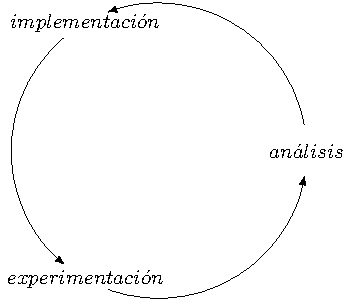
\includegraphics[width=0.5\textwidth]{applied-ci-cycle}
	\caption[Ciclo de aplicación de soluciones basadas en \acrlong{ci}]{Ciclo de aplicación de soluciones basadas en \acrlong{ci}. Los sistemas inteligentes se conciben, se implementan y se prueba. En la fase de experimentación se determina cómo de bien o de mal lo está haciendo y cuales son las decisiones a tomar para el nuevo ciclo. Cuandto más rápido se puede realizar este ciclo, más soluciones se pueden probar, por ello el impacto de la mayor capacidad computacional y la optimización de las ténicas de entrenamiento es tan importante.}
	\label{fig:applied-ci-cycle}
\end{figure}

El adjetivo \textit{deep}, en el contexto de las redes (e.g. redes neuronales, redes de creencia, \ldots), donde se origina este término, se refiere a una red con más capas de lo habitual\sidenote{
	De aquí surge el nombre de \textbf{shallow network} o red superficial, en contraposición a \textbf{deep network} o red profunda.
} (normalmente más de dos o tres). Este tipo de capas, históricamente ha sido más difícil de entrenar, debido entre otras cosas a las técnicas de entrenamiento (donde los parámetros tendían a diluirse según se aumentaba el número de capas entre la entrada y la salida) o a la disponibilidad de conjuntos de datos, los cuales al no ser muy grandes, las redes grandes tendían a sobre especializarse. La Figura~\ref{fig:deep-learning-capabilities} introduce, con una ilustración un tanto informal, las capacidades del deep learning frente a las de los modelos entrenados antes de esta época.

\begin{figure}
	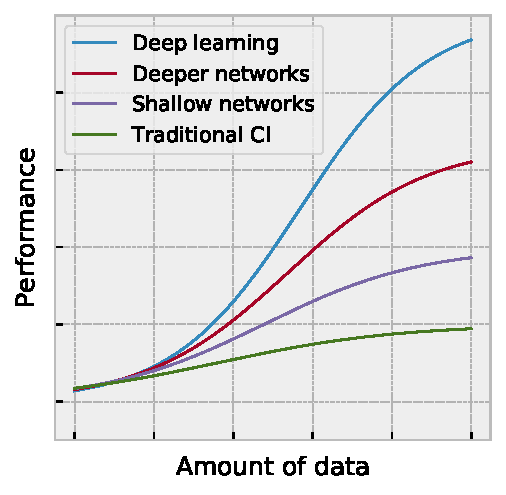
\includegraphics{deep-learning-capabilities}
	\caption[Capacidad de los modelos en función de la cantidad de datos]{La enorme cantidad de datos junto con la capacidad computacional y la mejora de las ténicas de entrenamiento hacen posible que en la actualidad, con las técnicas asociadas al contexto del deep learning, los modelos entrenados sean más eficientes  inteligentes. Imagen adaptada de la charla \textit{How scale is enabling deep learning} de Andrew Y. Ng, accesible \url{https://youtu.be/LcfLo7YP8O4}.}
	\label{fig:deep-learning-capabilities}
\end{figure}

Los factores antes mencionados han hecho posible la operación sobre redes más grandes y profundas con cantidades de ordenes de magnitud muy superiores. El resultado en la actualidad es que tenemos modelos que mejoran mucho los modelos anteriores, y no parece haber cota superior en su capacidad de aprendizaje\sidenote{
	Dentro de un contexto de aplicación específica, creemos que aún estamos muy lejos de crear vida inteligente.
}.


\section{\acrlongpl{ann}}

Son herramientas que tratan de replicar las funciones cerebrales de un ser vivo de una manera muy fundamental, esto es, desde sus componentes más básicos, las neuronas. Para ello se basan en estudios de neurobiología y de ciencia cognitiva moderna del cerebro humano\sidenote{
	Aún apoyándose en la topología y funcionamiento del cerebro humano para realizar el símil, lo cierto es que dichos modelos distan aún de considerarse \textit{cerebros artificiales}. La red neuronal más compleja hasta la fecha es la propuesta en~\cite{TraskANDREWTRASK}, con alrededor de $160.000$ parámetros a ser ajustados (podemos abstraernos y pensar en ellos como conexiones entre neuronas). Si comparamos esta cifra sólo con las del neocórtex (figura~\ref{fig:neocortex}) hace que, tecnológicamente hablando, nos quedemos con la sensación de estar aún a años luz de aproximarnos a la complejidad de un cerebro humano.
}.

Una \gls{ann} es independiente del problema a solucionar. Se la puede considerar como una caja negra que aprende las relaciones que subyacen en los datos de un problema para abstraer el modelo a partir de éstos. Estas características de aprendizaje y abstracción son los factores determinantes por los que son usadas en prácticamente todas las áreas de la ciencia y de la ingeniería (\cite{Du2006}).

\begin{figure}[t]
	\centering
	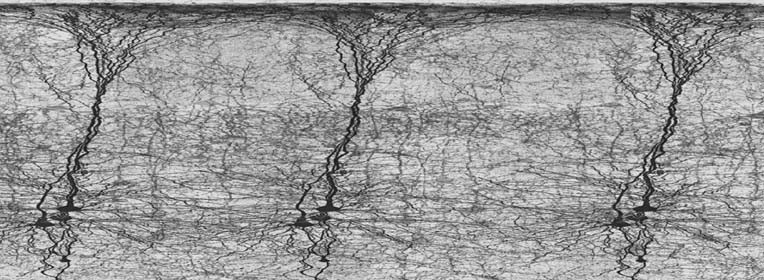
\includegraphics{neocortex}
	\caption[Ilustración de una sección del neocórtex humano]{Sección del neocórtex humano, región asociada a las capacidades cognitivas y que supone alrededor de un $76\%$ del volumen total del cerebro humano. Está distribuído en $6$ capas y miles de columnas que las atraviesan, cada una con alrededor de $10.000$ neuronas y un diámetro de $0.5mm$.  Como dato anecdótico, se estima que sólo en el neocórtex humano existen alrededor de $20.000$ millones de neuronas, cada una de las cuales conectada a entre $100$ y $100.000$ neuronas vecinas (\cite{Pakkenberg1997}). Esto supone entre $2 \cdot 10^{12}$ y $2 \cdot 10^{15}$ conexiones. Fuente: \textit{Blue Brain Project EPFL}, \url{http://bluebrain.epfl.ch/}.}
	\label{fig:neocortex}
\end{figure}

El primer trabajo en la disciplina se le atribuye a  los investigadores McCulloch-Pitts por su modelo de neurona artificial ilustrado en la figura~\ref{fig:mccullocs-pitts-neuron-model} (\cite{McCulloch1943}). Existen diferentes tipologías y formas de operar con redes, pero todas funcionan de la misma manera: unidades (e.g. neuronas) interconectados mediante enlaces por los que fluye la información de manera unidireccional, donde algunas de dichas unidades sirven de entrada al sistema (i.e. entradas o sensores), otras sirven de salida del sistema (i.e. salidas y actuadores) y otras como elementos internos (i.e. ocultas), y donde los pesos de sus conexiones se ajustan mediante un proceso denominado \textit{entrenamiento}, imitando los principios de la teoría hebbiana~\cite{hebb19680}.

\begin{figure}
	\centering
	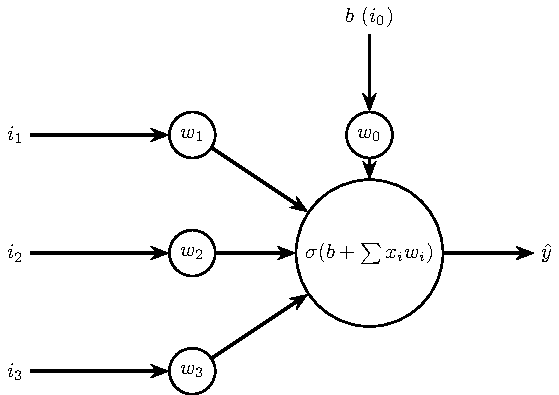
\includegraphics{artificial-neuron-model}
	\caption[Modelo de neurona artificial de McCulloch y Pitts]{Variación de la representación del modelo de neurona artificial propuesto por McCulloch y Pitts. En éste, cada una de las entradas $x_i$ es incrementada o inhibida aplicando el producto con su peso asociado $w_i$. La activación vendrá determinada por la aplicación de una función (denominada \enquote{de activación}) a la suma de los valores. Esta variación en concreto incluye una entrada $x_0$ y un peso $w_0$ como bias de la neurona para la variación dinámica del umbral de activación.}
	\label{fig:mccullocs-pitts-neuron-model}
\end{figure}

Este primer modelo de neurona proponía una función escalón para determinar si la neurona se activaba o no, como analogía del funcionamiento de la neurona artificial. Sin embargo, este modelo es muy limitado. La verdadera potencia de las redes surge del tanto del uso de funciones de activación no lineales como de la agrupación de estas neuronas en estructuras más complejas.

\subsection{Funciones de activación}

El valor de salida de una neurona queda determinado por la aplicación de una función sobre la entrada neta a ésta. Esta función dictamina el grado de activación de la neurona y para un correcto funcionamiento de la red en términos generales debe ser no lineal\sidenote{
	Supongamos una red neuronal con una estructura como la siguiente:
	
	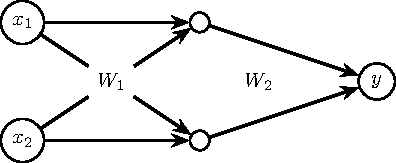
\includegraphics{mlp-linear}
	
	Supongamos, además, la función de activación de las neuronas es lineal (e.g. $f(x) = x$). La salida se puede expresar como:
	
	\begin{align*}
		\mathbf{y^1} = f(W_1 * \mathbf{x} + \mathbf{b_1}) \\
		y =  \mathbf{y^2} = f(W_2 * \mathbf{y^1} + \mathbf{b_2}) \\
	\end{align*}
	
	Por tanto:
	
	\begin{align*}
		y &= f(W_2 * f(W_1 * \mathbf{x} + \mathbf{b_1}) + \mathbf{b_2}) \\
		&= (W_2 * W_1) * \mathbf{x} + (W_2 \cdot \mathbf{b_1} + \mathbf{b_2}) \\
		&= W' * \mathbf{x} + \mathbf{b'} \\
	\end{align*}
	
	
	Siendo $\mathbf{y^l}$ el vector columna de salida de la capa $l$, $\mathbf{b_l}$ el vector de los bias de la capa  $l$ y $\mathbf{x}$ el vector columna de las entradas.
	
	Es decir, usando funciones lineales da igual el número de capas que tengamos, ya que la composición de dos funciones lineales es siempre una función lineal y la arquitectura se reducirá a una única capa de activación lineal. Por ello no tiene demasiado sentido el uso de funciones lineales en las capas ocultas de una red.
}.

Las funciones de activación clásicas usadas en redes neuronales han sido la función sigmoidal (eq.~\ref{eq:sigmoid}) y la tangente hiperbólica (eq.~\ref{eq:tanh}). Por un lado, son funciones no lineales que mantienen normalizados las activaciones de las neuronas, y por otro, son derivables a lo largo de todo el dominio de los reales, siendo su derivada además fácilmente computable. En la Figura~\ref{fig:sig-and-tanh} se muestra una representación gráfica de éstas funciones junto con su derivada.

\begin{equation}
\sigma (x) = \frac{1}{1+e^{-x}} \qquad
\frac{d\sigma (x)}{d(x)} = \sigma (x)\cdot (1-\sigma(x)).
\label{eq:sigmoid}
\end{equation}

\begin{equation}
\tanh(x) = \frac{e^x - e^{-x}}{e^x+e^{-x}} \qquad
\frac{d\tanh (x)}{d(x)} = 1 - \tanh^2(x)
\label{eq:tanh}
\end{equation}

\begin{figure}
	\centering
	\subfloat[]{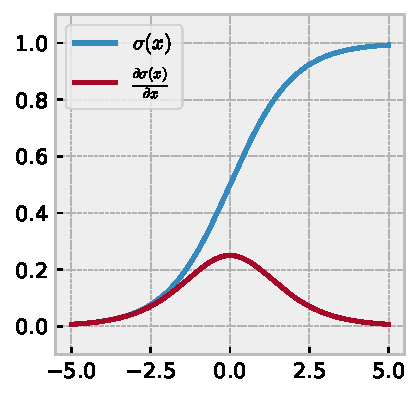
\includegraphics[width=0.46\linewidth]{sigmoid-function}}\qquad
	\subfloat[]{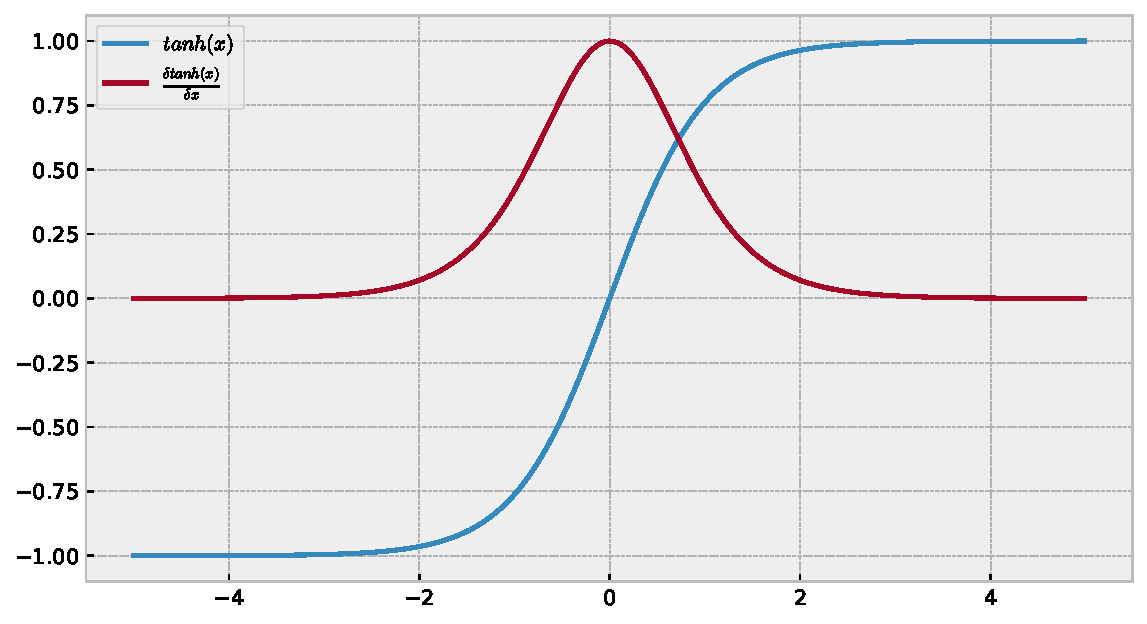
\includegraphics[width=0.46\linewidth]{tanh-function}}
	\caption[Funciones de activación: sigmoidal y tangente hiperbólica.]{Las funciones de activación sigmoidal y tangente hiperbólicas. Ambas se han usado como funciones de activación no lineales gracias a que sus derivadas son continuas a lo largo de todo el dominio y además son fácilmente computables.}
	\label{fig:sig-and-tanh}
\end{figure}

En general, la tangente hiperbólica es superior a la sigmoidal en todos sus aspectos. Computacionalmente es menos costoso el cálculo de una función sigmoidal, pero con la potencia de cómputo actual esta diferencia puede considerarse despreciable. Además de tener una forma similar a la sigmoidal, latangente hiperbólica permite enviar señales de activación negativas. Además, tiende a centrar los datos de una capa a otra en lugar de mantener un sesgo hacia el $0.5$ (recordemos que mientras que la sigmoidal está definida en el intervalo $(0, 1)$, la tangente hiperbólica se encuentra definida entre los intervalos $(-1, 1)$. Por tanto, en un caso general, la tengente hiperbólica suele ser preferible a la sigmoidal.

Aún así, en algunas situaciones sí podría tener sentido el uso de funciones sigmoidales en lugar de tangentes hiperbólicas. Por ejemplo, en un problema de clasificación, mantener en la capa de salida funciones de activación sigmoidales permite ajustar la salida en el intervalo $(0, 1)$, sin necesidad de realizar una posterior normalización.

Sin embargo, el principal problema de estas funciones es cuando los valores netos de las entradas son muy grandes. En ese caso, las funciones se acercan a los extremos, aproximándose sus gradientes a 0, y por tanto frenando el aprendizaje. Este error es denominado frecuentemente como \textit{vanishing gradient} en la literatura. Es una de las razones por las que en la fase de inicialización de una red neuronal se tendía a valores en torno al 0 en los pesos. Unos valores altos hacían que las entradas netas fuesen muy grandes ralentizando el aprendizaje.

\begin{figure}
	\centering
	\subfloat[]{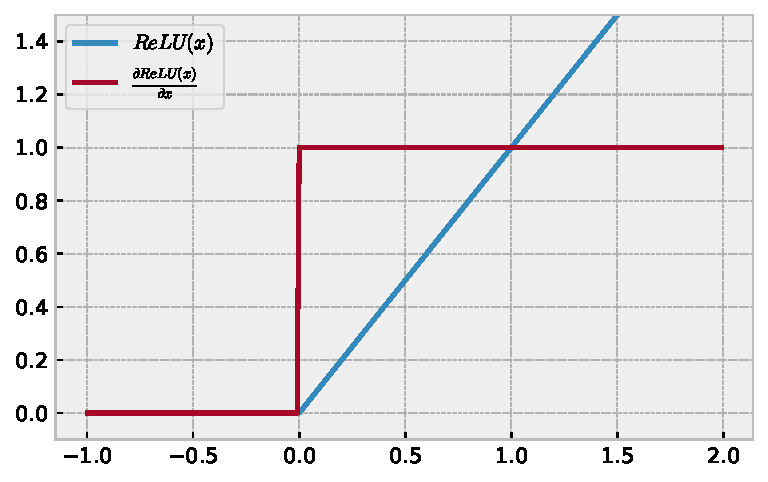
\includegraphics[width=0.46\linewidth]{relu-function}}\qquad
	\subfloat[]{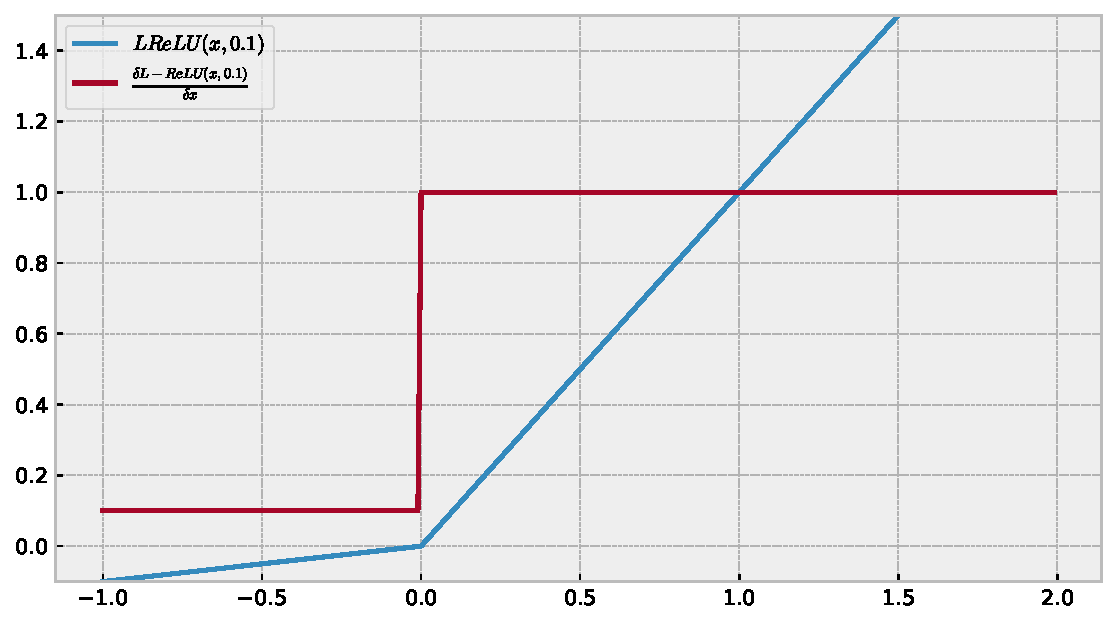
\includegraphics[width=0.46\linewidth]{leaky-relu-function}}
	\caption[Funciones de activación: \acrshort{relu} y Leaky-\acrshort{relu}.]{La función de activación (a) \gls{relu} evita el problema del estancamiento cuando la entrada neta de la neurona es muy alta. La función de activación \textit{Leaky} \gls{relu} (en este ejemplo, con $\epsilon = 0.1$) es una de las posibles soluciones cuando se permite que la entrada neta a la red sea menor que 0, ya que en el caso de la función \gls{relu} la derivada es 0 y por tanto el gradiente no nos indica hacia dónde ha de descender el error.}
	\label{fig:relu-and-leaky-relu}
\end{figure}

Uno de los avances dentro del Deep Learning (ver~\ref{ss:deep-learning}) fue el uso de un tipo de función de activación denominada \acrfull{relu} (eq.~\ref{eq:relu}). Ésta posee una forma muy simple pero es increíblemente efectiva. Por un lado, evita el problema del \textit{vanishing gradient} dado que su derivada es constante en el intervalo $(0, \infty)$. Por otro, su cálculo es tremendamente simple comparado con el resto de funciones (no deja de ser un máximo). En la figura~\ref{fig:neocortex}

\begin{equation}
ReLU(x) = max(0, x) \qquad
\frac{d ReLU(x)}{d(x)} \approx
\begin{cases}
0 &\quad\text{if} x < 0 \\
1 &\quad\text{if} x \geq 0 \\
\end{cases}
\label{eq:relu}
\end{equation}

\begin{equation}
L-ReLU_\epsilon(x) = max(0, x) \qquad
\frac{d L-ReLU_\epsilon(x)}{d(x)} \approx
\begin{cases}
\epsilon &\quad\text{if} x < 0 \\
1 &\quad\text{if} x \geq 0 \\
\end{cases}
\label{eq:leaky-relu}
\end{equation}

Este tipo de neurona tiene una serie de características que merece la pena comentar:

\begin{itemize}
	\item No existe derivada en $0$. El aprendizaje, basado en el descenso del gradiente, se encuentra con una indeterminación en $0$. Sin embargo, es fácilmente subsanable incluyendo el valor 0 o 1 en la derivada en el punto 0. Aunque no es  matemáticamente correcto, computacionalmente se está reemplazando la derivada por una función muy aproximada al ésta en la que el algoritmo de descenso del gradiente se comporta de forma muy similar. Por ejemplo, la representación en la Figura~\ref{fig:relu-and-leaky-relu}, la derivada es $1$ en el punto $x = 0$.
	\item Sin límite superior y derivada $0$ para $x < 0$. Estas características pueden ser una ventaja o una desventaja. Las activaciones muy fuertes representan relaciones entre elementos muy próximos entre sí, aunque tienen el riesgo de anular el impacto del resto de entradas, pudiendo ralentiazr el aprendizaje. Por otro lado, en el momento que el gradiente de una neurona se hace 0, ésta \textit{\enquote{muere}}, pudiendo ser una desventaja ya que la red dispone de menos neuronas para representar un modelo, como una ventaja, al ajustarse el modelo al número de neuronas necesarias. En general, las desventajas en estos aspectos aparecen cuando el factor de aprendizaje es notoriamente alto.
\end{itemize}

Por último, la función de activación \textit{Leaky} \gls{relu} (eq.~\ref{eq:leaky-relu}) es una evolución de la \gls{relu} para el uso en problemas donde es ventajoso que una neurona no llegue a tener nunca un gradiente de 0. Van acompañadas de un parámetro $\epsilon \approx 0$ que determina la pendiente para todos aquellos valores menores de 0. Un ejemplo de esta neurona se ilustra en la figura~\ref{fig:relu-and-leaky-relu}. Su uso no está muy extendido, pero existen casos en los que su uso está justificado.

\subsection{Estructura y clasificación de redes neuronales}

Las \gls{ann} reciben ese nombre debido a que son sistemas formados por multitud de neuronas artificiales simples. Dependiendo de cómo su topología y configuración, éstas serán más adecuadas para unos u otros problemas (e.g. unas serán más adecuadas para regresión, clasificación, predicción, \textit{clustering}).

Típicamente, estas redes se componen de neuronas conectadas, por lo que se puede pensar en ellas como un grafo ponderado donde los nodos se corresponden a las neuronas, las aristas a las conexiones entre entradas y salidas y los pesos de las aristas a los pesos de las conexiones de entrada. Existen diferentes topologías o arquitecturas dependiendo de qué forma toma el grafo que modela las neuronas y sus conexiones. Estos dos tipos son los siguientes:

\begin{itemize}
	\item Redes \textbf{feed-forward} (o prealimentadas). Sus representación como grafo no presenta ningún ciclo (por tanto ninguna retroalimentación entre neuronas, como se ilustra en la figura~\ref{fig:ff-vs-rnn}). Es la topología más usada en aplicaciones prácticas debido a su sencillez y su efectividad. En ellas el flujo de información sigue un camino desde un conjunto de neuronas denominadas \textit{entradas} hasta otro conjunto de neuronas denominado \textit{salidas}. No es requisito que las neuronas se agrupen en capas, aunque suele ser la estructura común. A las redes de más de dos/tres capas ocultas (i.e. las capas que se encuentran entre la capa de neuronas de entrada y la capa de neuronas de salida) se las suele denominar \textit{profundas} o \textit{deep}. Representantes clásicos de esta categoría pueden ser el \gls{mlp}~\cite{rumelhart1985learning}, los autoencoders~\cite{Hinton2006} o los \gls{som}~\cite{kohonen1998self}.
	\item Redes \textbf{recurrentes}. Éstas, a diferencia de las prealimentadas, tienen al menos un ciclo dentro de su representación, de tal manera que el flujo de información de salida de una neurona puede llegar a afectar a su propio estado. Aunque estas topologías representan de una forma más fiel las bases biológicas de las \gls{ann}, históricamente han sido más complejas a la hora de operar y entrenar debido a sus relaciones entre nodos. Sin embargo, durante la última década han aparecido nuevas técnicas que facilitan su operación. Algunos casos particulares de este tipo de arquitectura son las Redes de Hopfield~\cite{hopfield1982neural} o las redes \gls{lstm}~\cite{hochreiter1997long}.
\end{itemize}

\begin{figure}[t]
	\centering
	\subfloat[]{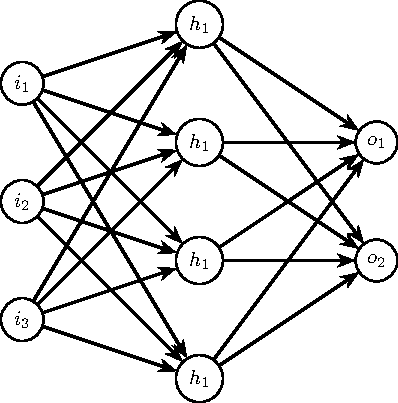
\includegraphics[width=0.46\linewidth]{multilayer-perceptron}}\qquad
	\subfloat[]{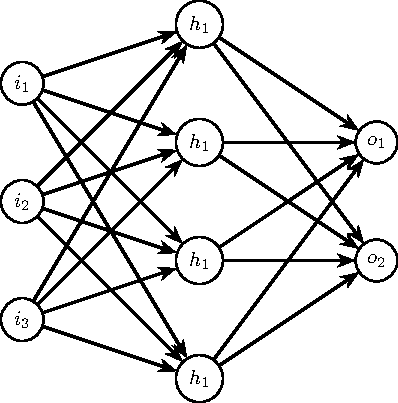
\includegraphics[width=0.46\linewidth]{multilayer-perceptron}}
	\caption[Diferencias entre toppologías de redes \textit{feed-forward} y \textit{recurrentes}]{Diferencias entre los grafos que representan las \acp{ann} de tipos (a) \textit{feed-forward} y (b) recurrentes. Las redes recurrentes presentan ciclos entre sus nodos que permiten la retroalimentación interna entre las neuronas. Suelen ser más útiles a la hora de modelar eventos en el tiempo, aunque su entrenamiento es más complejo.\TODO{CAMBIAR LA FIGURA DE LA RECURRENTE}}
	\label{fig:ff-vs-rnn}
\end{figure}

Esta tesis se centra en redes pertenecientes al primer grupo, concretamente en las topologías \gls{mlp} y \gls{cnn}, con las que se cerrará la presente sección. Ambos tipos de redes han probado su efectividad en diferentes dominios, aunque las segundas están demostrando su efectividad con las nuevas ténicas surgidas a partir del \textit{deep learning}

\subsection{Perceptrones multicapa}

En un perceptrón multicapa, las neuronas se encuentran agrupads en capas de tal manera que todas las salidas de las neuronas de una capa se conectan a todas las entradas de cada una de las neuronas de la capa siguiente. A las primera y últimacapas de la red se las denomina respectivamente capa de entrada y de salida, mientras que las capas intermedias son denominadas capas ocultas. Hemos visto algunasilustraciones a lo largo del presente capítulo, pero en la Figura~\ref{fid:detailed-multilayer-perceptron} se puede ver en detalle este tipo de red.

La forma de calcular la salida de un perceptrón multicapa es la siguiente. Supongamos que tenemos dos capas, $l-1$ y $l$, compuestas por $n^{l-1}$ y $n^l$ neuronas respectivamente cada una con su función de activación $f$, y como conexiones (pesos) entre ambas capas tendremos una matriz $W^l$ de dimensiones $(l-1, l)$. Cada una de las neuronas deberá tener una entrada de bias, por lo que tendremos tambien un vector columna $\mathbf{b}^l$ que los representará. La salida $\mathbf{s}^l$ de esa capa será un vector columna que se obtendrá a partir de la siguiente función que se muestra en la ecuación~\ref{eq:ff-mlp}:

\begin{equation}
	\mathbf{s}^l = f(W^l \mathbf{s}^{l-1} + \mathbf{b}^l)
	\label{eq:ff-mlp}
\end{equation}

Como se puede observar, la salida $s^l$ de la capa $l$ depende directamente de la salida de la capa $l - 1$. El proceso de calcular la salida es incorporando las entradas en la capa de entrada e ir iterando hasta la capa de salida.

El algoritmo base de aprendizaje en un perceptrón multicapa de denomina \textit{back-propagation}~\cite{rumelhart1985learning} y se basa en la regla delta~\cite{widrow1960adaptive} para el perceptrón simple. Éste usa una técnica denominada \textit{descenso del gradiente} donde lo que se intenta es minimizar el valor de una función $f(x)$ que representa el error (en realidad el \textit{coste}\sidenote{
	Existen dos términos asociados al error en \glspl{ann}: el error y el coste, que en la literatura se denominan \textit{loss} y \textit{cost} respectivamente. El primero se refiere al error existente entre la salida de la red neuronal y la salida esperada de un ejemplo en concreto, mientras que el segundo se refiere al error sobre todo el conjunto de entrenamiento. Es de esperar que durante el proceso de entrenamiento este error baje.
	
	Existen diferentes funciones para calcular el error y el coste de un modelo en concreto. En el caso del coste, lo más común es usar la media entre todo el conjunto de entrenamiento como:
	
	\begin{equation*}
		C(M) = \frac{1}{m} \sum_{i=1}^m L(\hat{y}_i, y_i)
	\end{equation*}
	
	Donde $M$ es el modelo actual, $m$ el número total de ejemplos y $L$ la función de error entre las salidas $\hat{y}$ e $y$ de cada ejemplo $i$. En algunos casos se usa la media ponderada para dar más importancia a determinados casos, pero no es lo común.
	
	Sin embargo, en el caso del error, existen varias funciones dependiendo de cuál sea la tarea. Por ejemplo, para tareas de regresión, lo común es usar el error cuadrático medio o su raíz cuadrada. Para tareas de clasificación, una función de error muy útil que ha remplazado a la función $hit$ ()relación de aciertos-fracasos) es la entropía cruzada, que tiene la siguiente forma:
	
	\begin{equation*}
		L(\hat{y}_i, y_i) = (1 - y) \log (1 - \hat{y}) - y \log \hat{y}
	\end{equation*}
	
	La razón es que en esta última se capturan sutilezas como lo cercano que ha estado un acierto. Por ejemplo, si nuestro objetivo es una salida de clasificación $(1, 1, 0)$ y tenemos dos modelos, uno que dice $(0.9, 0.9, 0.6) \rightarrow (1, 1, 1)$ y otro que dice $(0.6, 0.6, 0.6) \rightarrow (1, 1, 1)$, según la función hiy, ambos modelos funcionan igual mientras que según la entropía cruzada el primero funciona mejor que el segundo.
	
	Curiosamente, la entropía cruzada también funciona bien en problemas de regresión, aunque es más sencillo interpretar los resultados de un $RMSE$ y por tanto su uso no está extendido.
}) de la red calculando como aumenta o disminuye esta con peqñeas variaciones de $x$.

El algoritmo trata de aplicar un error desde la salida de la red sobre todos los pesos de la misma en función de cuánto han colaborado en dicho error (bajo la suposición de que, cuando mayor es un error, más ha contribuido). El problema es cómo se calcula este error. En la última capa es sencillo (conocemos las salidas real y esperada), pero la genialidad del algoritmo es que el error en las interiores lo determina a partir del error de las sucesivas capas apoyándose en el descensodel gradiente. Es decir:

Supongamos que nos encontramos en la capa $l$ para la cual conocemos el error de salida que denotaremos como el vector columna $\delta \mathbf{s}^l$, y donde todas las neuronas usan la función de activación $f$. Entonces, de acuerdo al gradiente, el error neto que produce nuestra salida se corresponde con:

\begin{equation}
	\delta \mathbf{e} = \delta \mathbf{s}^l \circ f'(W^l \cdot \mathbf{s}^{l-1} + \mathbf{b}^l)
\end{equation}

Nótese que $\circ$ denota al producto de Hadamard (elemento a elemento). También es interesante fijarse en que $W^l \cdot \mathbf{s}^{l-1} + b^l$ se corresponde al cálculo de la entrada neta de la capa $l$ antes de aplicarle la función de activación $f$.

Una vez conocido este error podemos pasar a calcular cómo varían los parámetros de la capa (eq.~\ref{eq:bp-weights} y~\ref{eq:bp-bias}) y el error de salida (eq.~\ref{eq:error-previous-layer}) de la capa anterior de la siguiente manera:

\begin{subequations}
	\begin{equation}
		\delta \mathbf{s}^{l-1} = W^{l\top} \cdot \delta \mathbf{e} \label{eq:error-previous-layer}
	\end{equation}
	\begin{equation}
		\delta W^l = \delta \mathbf{e} \cdot \delta \mathbf{s}^{l-1} \label{eq:bp-weights}
	\end{equation}
	\begin{equation}
		\delta \mathbf{b}^l = \delta \mathbf{e} \label{eq:bp-bias}
	\end{equation}
\end{subequations}

El valor $\delta \mathbf{s}^{l-1}$ será el valor de entrada para la capa anterior, mientras que los valores $\delta W^l$ y $\delta b^l$ serán los gradientes calculados. La forma máscomúnde aplicar el error es la que se muestra en las ecuaciones~\ref{eq:error-applied-to-weights} y~\ref{eq:error-applied-to-bias}:

\begin{subequations}
	\begin{equation}
		W^l = W^l + \alpha \delta W^l \label{eq:error-applied-to-weights}
	\end{equation}
	\begin{equation}
		\mathbf{b}^l = \mathbf{b}^l + \alpha \delta \mathbf{b}^l \label{eq:error-applied-to-bias}
	\end{equation}
\end{subequations}

Esta es la forma original del algoritmo de back propagation. Al valor $\alpha$ que aparece en las ecuaciones se le denomina factor de aprendizaje y como se puede apreciar, su valor determina lo rápido que cambian los pesos. Suele tomar valores entre $0.1$ y $0.01$, pero dependiendo de la evolución del entrenamiento y de la variación del algoritmo, éste puede llegar a tomar valores mucho más bajos. Algunas de las variaciones sobre el algoritmo inicial son las siguientes:

\begin{itemize}
	\item \textbf{Momento de inercia}~\cite{qian1999momentum}. Al algoritmo se le añade un factor por el cual los movimientos en el mismo sentido durante sucesivos epochs se acumulan. De esta manera, elriesgo de caer en mínimos locales disminuyen al ser capaz el algoritmo de \enquote{saltar} pequeños baches.
	\item \textbf{Adagrad}~\ref{duchi2011adaptive}, \textbf{RMSProp}~\ref{tieleman2012lecture} y \textbf{Adadelta}~\cite{zeiler2012adadelta}. Los tres se basan en el mismo principio. Al factor de entrenamiento de la red se le añade la existencia de un factor de entrenamiento por cada peso de tal manera que se actualiza de forma diferente en función de la evolución de su gradiente individual.
	\item \textbf{Adam}~\cite{kingma2014adam}. Este algoritmo combina los funcionamientos del momento junto con los del gradiente adaptativo del algoritmo RMSProp. Es el más utilizado en los últimos años.
\end{itemize}

\subsection{Redes de convolución}

Tal y como su nombre indica, las \acp{cnn} son redes que usan convouciones para su funcionamiento. Aunque también está estructurada en capas, su funcionamiento es diferente. Para comenzar, su estructura se puede dividir en dos regiones bien diferenciadas, una que se dedica a la extracción de características de la entrada (la denominaremos \textit{extracción de patrones}) y otra que se dedica a la clasificación o regresión de la entrada a partir de las características extraídas (que denominaremos \textit{predicción}). En la Figura~\ref{fig:cnn-general-structure} podemos ver una ilustración del esquema general de una \acl{cnn} donde se identifican ambas regiones.

\begin{figure}
	\missingfigure[figheight=4cm]{Ilustración con las dos formas de razonamiento}
	\caption[Estructura general de una \acl{cnn}]{Estructura general de una \acl{cnn}. Se pueden observar sombreadas de distinto color la relación existente entre las regiones de identificación de patrones y la de predicción. La primera actua sobre la entrada extrayendo características consideradas relevantes mientras que la segunda tranaja sobre esas características en lugar de sobre todo el espacio de entrada.}
	\label{fig:cnn-general-structure}
\end{figure}

La región de inferencia es en esencia un \ac{mlp}. A éste le llega un conjunto de entradas deducidas en la región anterior y realiza la operación de regresión o de clasificación que le corresponda. El funcionamiento se explica en el apartado anterior dedicado a este tipo de redes. La región de extracción de patrones es más interesante y merece más contenido.

\paragraph{Convoluciones}

Una convolución es una operación matemática que funciona como filtro sobre una estructura espacial (en este contexto, normalmente de matriz o de cubo) para identificar patrones y/o para transformar estructuras identificadas. Para simplificar la explicación en este apartado, supondremos que la entrada se trata de una matriz bidimensional (e.g. una imagen de un sólo canal de color), y que los filtros son también bidimensionales, pero es común tener espacios de entrada de más dimensiones\sidenote{
	De hecho, para analizar imágenes lo normal es trabajar sobre los diferentes canales de color como capas diferentes, por lo que una imagen es en realidad una matriz tridimensional de dimensiones $(w, h, c)$ donde $w$ es el ancho, $h$ es el alto y $c$ es el número de canales.
	
	\centering
	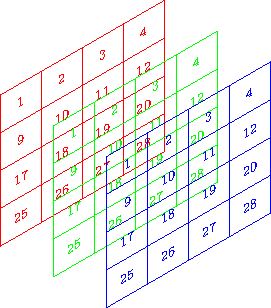
\includegraphics[width=0.46\linewidth]{three-channels-for-an-image}
}. La ecuación~\ref{eq:convolution-example} describe el resultado de aplicar una convolución de un filtro sobre una matriz.

\begin{equation*}
	\begin{pmatrix}
		8 & 7 & 4 & 7  \\
		0 & 1 & 1 & 3  \\
		3 & 4 & 7 & 1  \\
		5 & 2 & 5 & 0
	\end{pmatrix}
	\circledast
	\begin{pmatrix}
		1 & 0 &  \\
		0 & 1
	\end{pmatrix}
	=
	\begin{pmatrix}
		9 & 8 & 7  \\
		4 & 8 & 2  \\
		5 & 9 & 7
	\end{pmatrix}
	\label{eq:convolution-example}
\end{equation*}

El símbolo $\circledast$ denota la operación de convolución. Esta operación hacer recorrer el filtro por todas las posiciones hasta que recubre todo el espacio inicial\sidenote{
	La operación básica recorre las posiciones una a una. Existe un parámetro, denominado \textit{stride} que puede modificar este comportamiento. Nosotros nos ceñiremos a un stride de tamaño $1 \times 1$ para simplificar el discurso.
}. Para cada posición, se realizará el sumatorio del producto elemento a elemento, y el resultado se asignará en dicha posición. Esto implica que el tamaño de la matriz resultante es inversamente proporcional al tamaño del filtro. Concretamente, si $(M_w, M_h)$, $(F_w, F_h)$ y $(R_w, R_h)$ son el ancho y el alto para las matrices origen, filtro y resultado, se cumple que:

\begin{align}
	R_w = M_w - F_w + 1 \\
	R_h = M_h - F_h + 1
	\label{eq:convolve-result-sizes-basic}
\end{align}

No obstante este funcionamiento de las convoluciones tiene un problema: las matrices tienden a ser cada vez más pequeñas con cada opreación de convolución. En el contexto del \textit{deep-learning}, el número de capas es finito y viene determinado por el tamaño del filtro.

La solución a este problema es la aplicación de una técnica denominada \textit{padding} que aumenta la matriz de origen para que la matriz resultante tras la operación de convolución quede del mismo tamaño\sidenote{
	En general, el padding genera la cantidad de celdas con 0 alrededor de la imagen para que a la hora de aplicarlo el resultado sea igual. Es una solución válida, pero dependiendo del problema puede interesar usar diferentes formas de padding. Por ejemplo, en nuestro problema, el cálculo de los valores de padding horizontal es diferente. En la parte dedicada al desarrollo de la tesis se explicará el cálculo y el por qué.
}. El cálculo del tamaño del padding para que la matriz resultado sea del mismo tamaño deberá ser:

\begin{align}
	P_w = \frac{F_w - 1}{2} \\
	P_h = \frac{F_h - 1}{2} 
	\label{eq:convolve-filter-padding-dims}
\end{align}

Por tanto es necesario que los filtros sean de dimensión impar.

\paragraph{Capas de convolución}

Las capa más importante en una \ac{cnn} son las capas de convolución. Éstas se componen de un número variable de filtros que representan las características que queremos extraer de la matriz de entrada. La entrada a esta capa de convolución será la matriz a la que aplicar los filtros, y la salida será una no linearización sobre el resultado de la convolución, modificándose en el proceso la dimensión de la matriz resultado. La figura~\ref{fig:convolution-layer} ilustra esto.

\begin{figure}
	\centering
	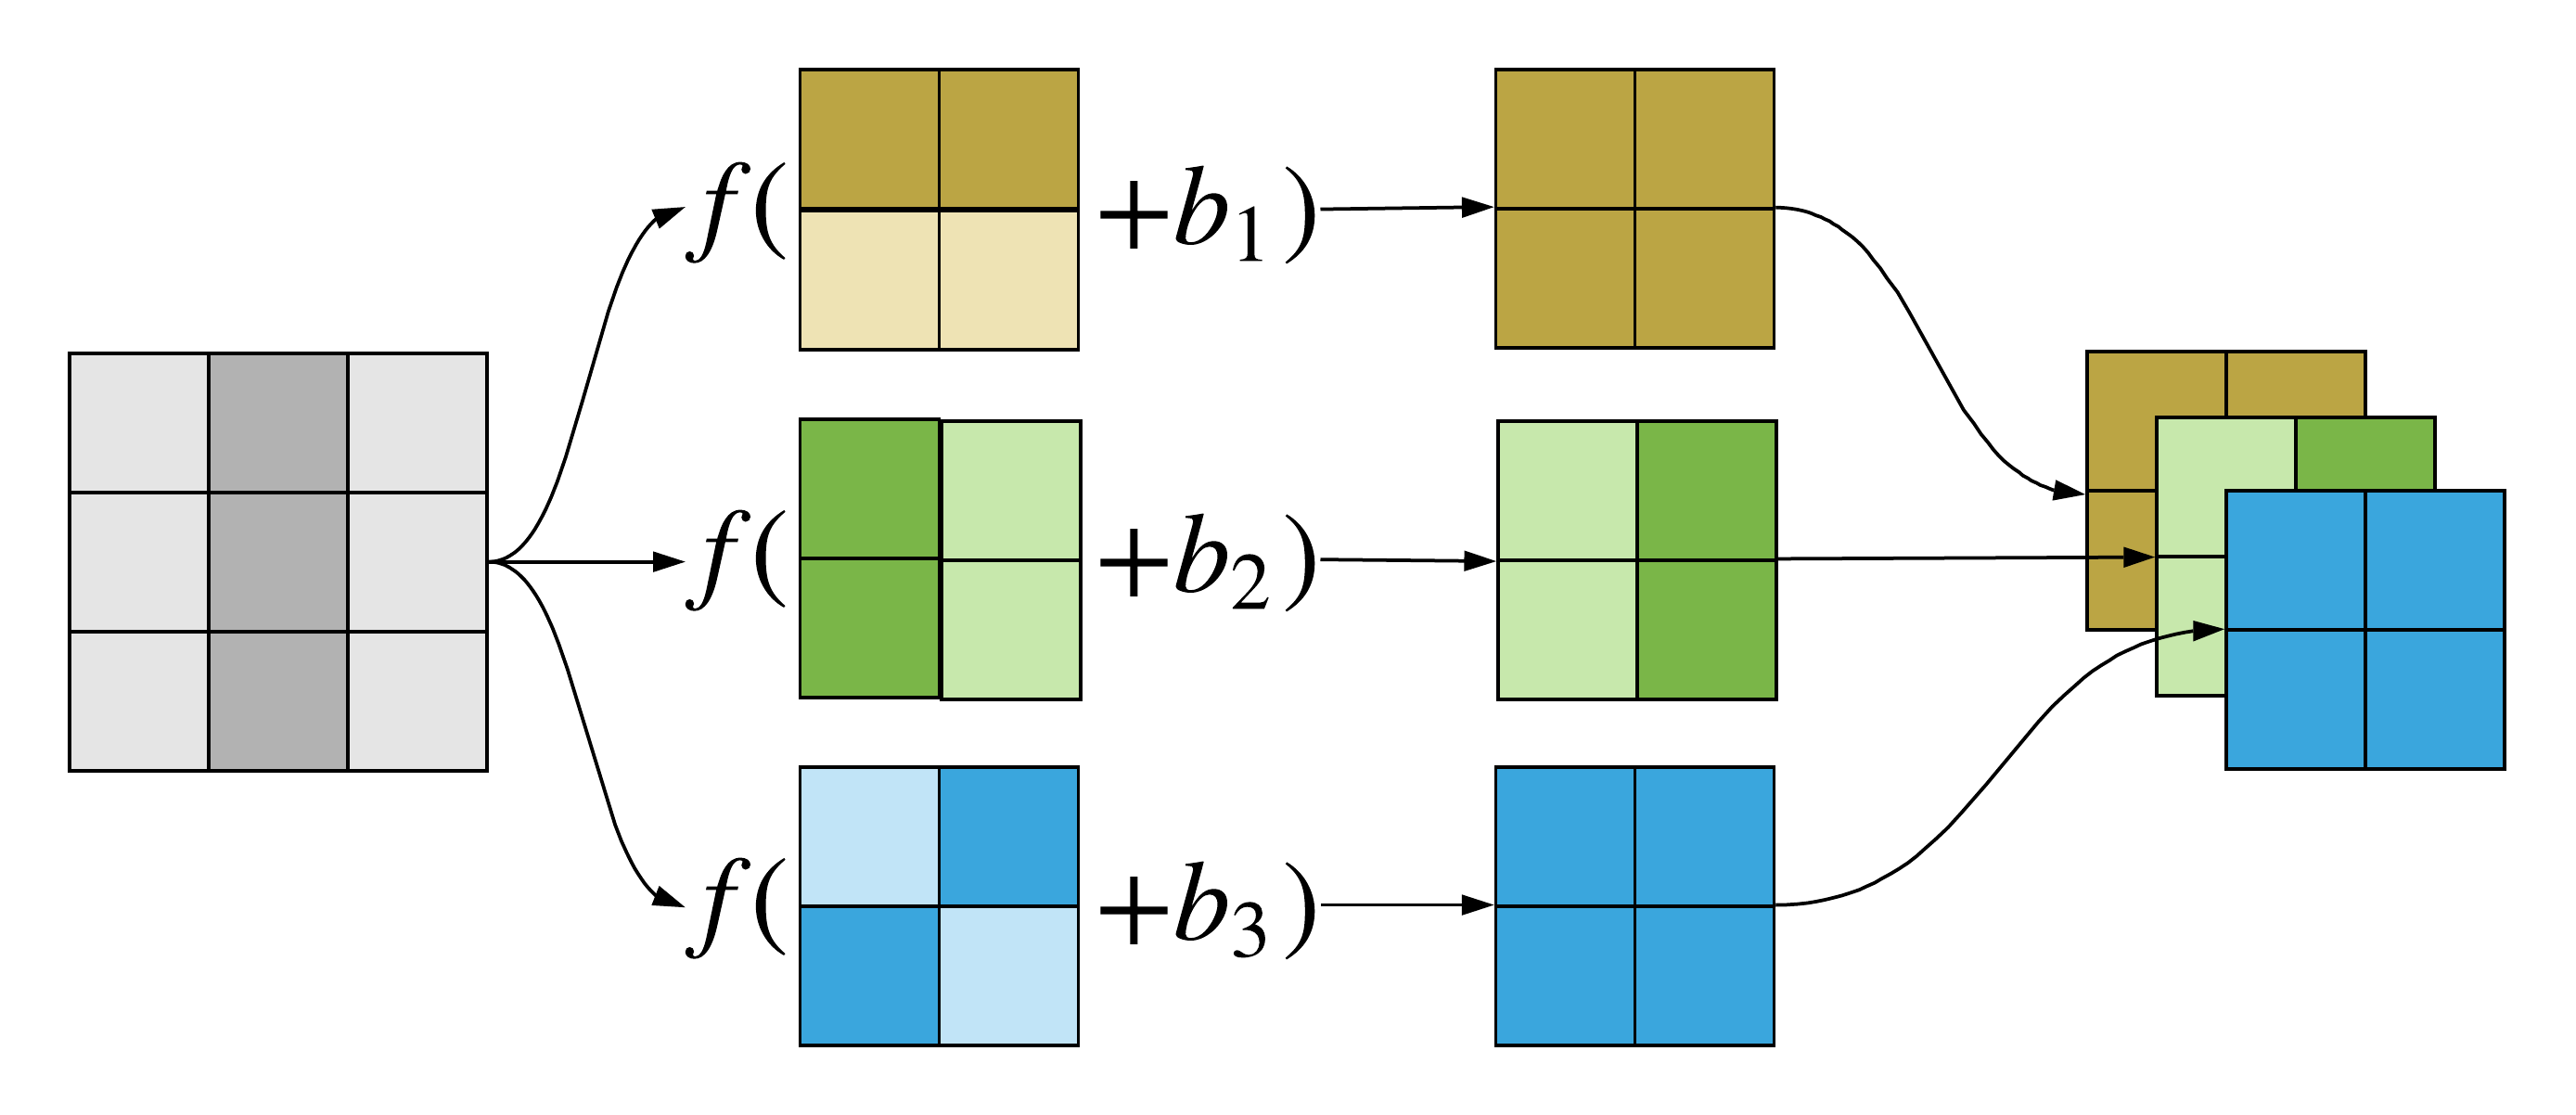
\includegraphics{convolution-layer}
	\caption[Descripción de la capa de convolución]{Descripción de la capa de convolución. Como entrada se recibe una matriz tridimensional con una capa de profundidad. Los filtros han de tener la misma profundidad, mientras que la matriz resultado tiene como profundidad el número de filtros. A las convoluciones (más un bias) se les aplica una función no lineal como en los \ac{mlp}. Por tanto, son los valores del filtro junto con los bias los parámetros que el algoritmo de aprendizaje debe aprender.}
	\label{fig:cnn-gconvolutional-layer}
\end{figure}

El proceso de aprendizaje en una red de convolución sin embargo no es trivial. Sigue apoyándose en el cálculo de los gradientes en función de los parámetros, que en este caso son los valores del filtro junto con un bias por cada filtro. Las ecuaciones de este cálculo en una capa bidimensional (para cada uno de los filtros) son las siguientes:

\begin{subequations}
	\begin{equation}
		\delta W_f = \sum_{w=0}^{F_h} \sum_{h=0}^{F_w} S^{l*} \times \delta C_{w,h} \label{eq:cnn-error-weights}
	\end{equation}
	\begin{equation}
		\delta b_f = \sum_{w=0}^{F_h} \sum_{h=0}^{F_w} \delta C_{w,h} \label{eq:cnn-error-biases}
	\end{equation}
\end{subequations}

En estas ecuaciones, $\delta C_{w,h}$ se refiere al gradiente del coste respecto a la salida de la capa de convolución correspondiente al filtro $f$ en la celda $(w, h)$. Así mismo, $S^{l*}$ se corresponde con la región (slice) de la entrada que se usó para calcular el correspondiente $\delta C_{w,h}$.

Etas ecuaciones son más complejas en función de cómo varía el número de filtros y de dimensiones de los mismos, pero al final usa los mismos principios que los \acp{mlp}.

\paragraph{Pooling y normalización}

Junto con las capa de convolución, normalmente se usan otros dos tipos de capa diferentes: las capas de \textit{pooling} y las de \textit{normalización}.

El \textit{pooling} es una operación de discretización del espacio de entrada. El objetivo es reducir las dimensiones de las entradas para las siguientes capas. Esto mejora el coste computacional y ayuda contra la sobre-especialización, ya que hay menos parámetros sobre los que trabajar para la misma entrada.


\begin{figure}
	\centering
	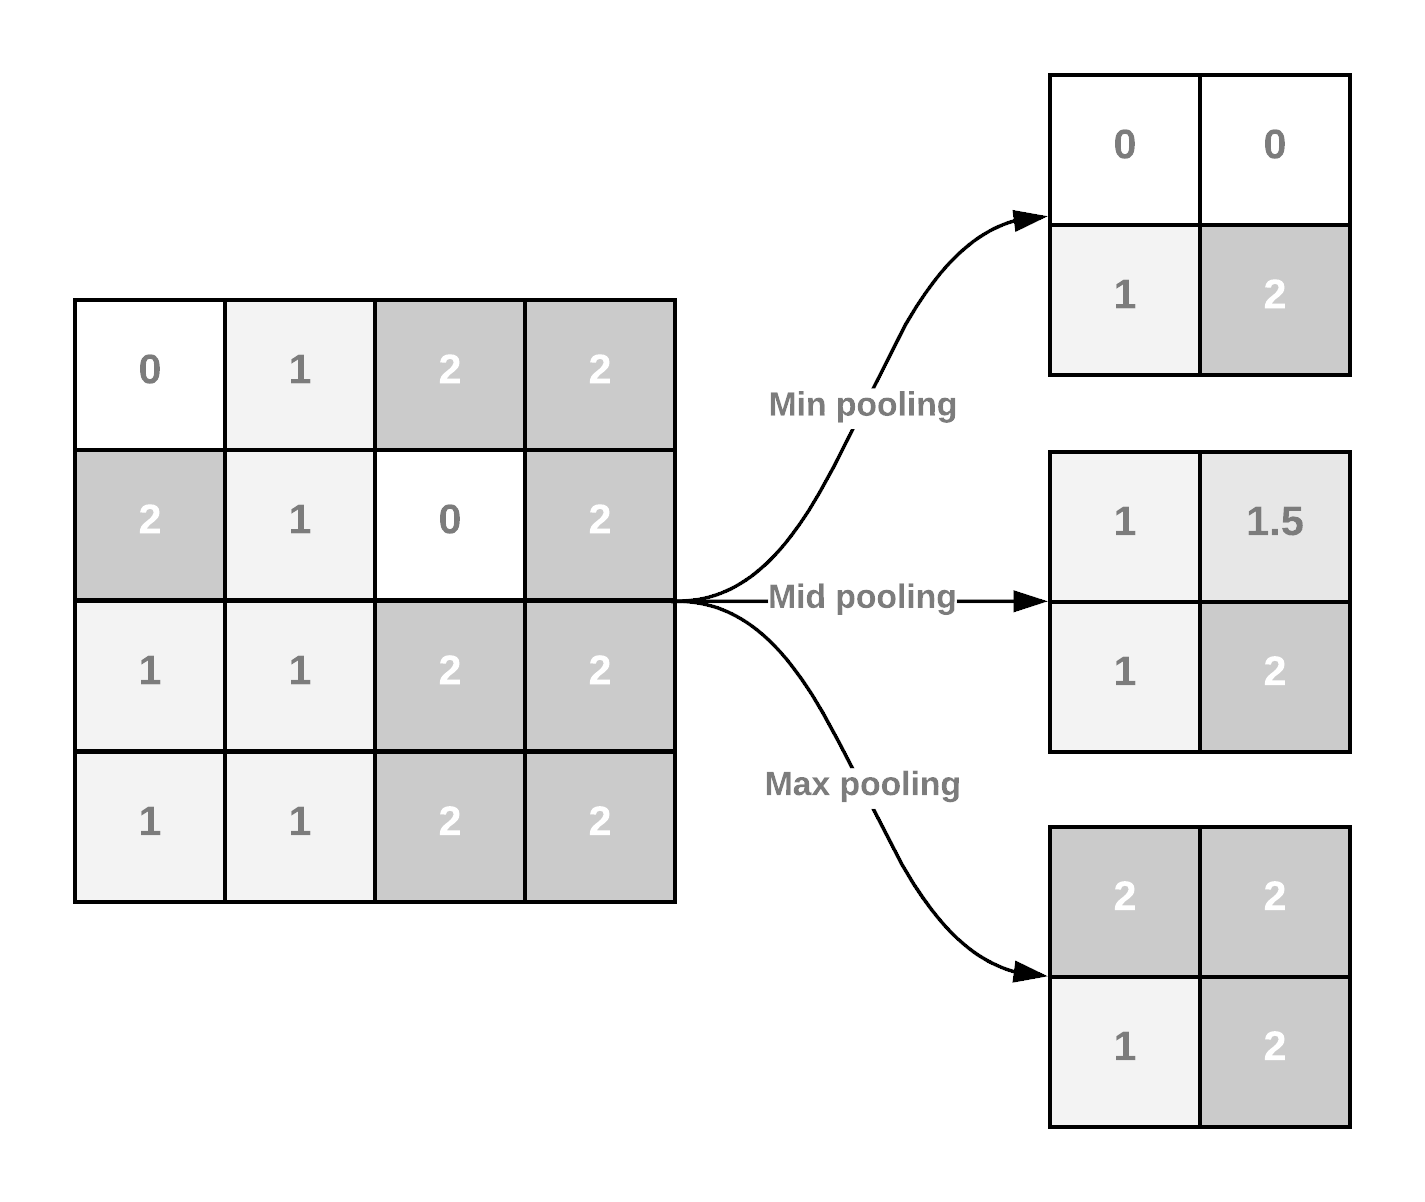
\includegraphics{cnn-pooling}
	\caption[Ejemplo de las operaciónes de \textit{pooling}.]{Ejemplo de las operaciónes de \textit{pooling} sobre una matriz de entrada de dos dimensiones. El filtro de tamaño $2 \times 2$ recorre la matriz en saltos de 2 celdas horizontales y 2 verticales extrayendo de cada región filtrada el mayor valor, el menor o el valor medio dependiendo de si la operación es \textit{max-pooling}, \textit{min-pooling} o \textit{mid-pooling}.}
	\label{fig:cnn-pooling}
\end{figure}

Su funcionamiento es similar al de las convoluciones (después de todo se tratan también de filtros), con la diferencia de que se mueven en ventanas no solapables devolviendo un valor para cada ventana y reduciendo por tanto el tamaño de la entrada. Existen tres tipos fundamentales que son el máximo, el mínimo y la media, y su diferencia estriba en el cálculo del valor de salida a partir de los valores de la entrada. En la Figura~\ref{fig:max-pooling} se ilustra un ejemplo de la operación de \textbf{max-pooling}\sidenote{
	Es curioso que por un lado se inventen mecanismos para mantener los tamaños de entradas-salidas entre convoluciones y luego no se use el comportamiento de las convoluciones con un \textit{stride} del tamaño del filtro para realizar esa reducción. De hecho existen algunos estudios que afirman que el uso del \textit{pooling} conlleva un aumento computacional sobre el uso de convoluciones para reducir el tamaño sin implicar una pérdida de rendimiento a la hora de predecir. Un ejemplo de esto lo tenemos en~\cite{howard2017mobilenets} donde afirman:
	
	\blockquote{We find that max-pooling can simply be replaced by a convolutional layer with increased stride without loss in accuracy on several image recognition benchmarks}
}.

La normalización es otra operación, esta a nivel de capa, que reafirma las diferencias entre los valores existentes en la matriz, similar a un aumento de contraste en una imagen. Permite destacar diferencias y en general los resultados demuestran que acelera el proceso de aprendizaje de una \ac{cnn} drásticamente cuando se incluye como capa oculta.

En los últimos años, los tipos más comunes de normalización son el \gls{lrn}~\cite{robinson2007explaining} y el \textit{batch normalization}~\cite{ioffe2015batch}.

\subsection{Solucionando los problemas de entrenamiento}

Anteriormente hablábamos de los problemas a los que se enfrentan los procesos de entrenamiento en la \gls{ci}. En líneas generales, los problemas de subespecialización pueden darse por tres razones diferentes:

\begin{itemize}
	\item La red no es lo suficientemente grande. Puede ocurrir que el conjunto de datos requiera de más propiedades o parámetros. Las solución es incrementar el número de capas o de neuronas por capa a fin de que el modelo acabe aprendiendo al menos los datos del conjunto de entrenamiento.
	\item El modelo no ha sido entrenado lo suficiente. Este caso es más raro, pero puede ser que el modelo sea lo suficientemente complejo para requerir más ciclos de entrenamiento. También puede ser que algunos hiperparámetros como el factor de entrernamiento o las funciones de activación están predisponiendo al modelo a aprender más lentamente.
	\item La topología del modelo no se adecúaa los datos. Puede ocurrir que el modelo que estamos tratando de aprender aprenda mucho mejor en una topologías que en otras. Por ejempo, para aprender a clasificar imágenes, las \glspl{cnn} funcionan mejor, entre otra serie de razones, porque mantiene una coherencia espacial entre los píxeles de la imagen desde el principio, cosas que con un \gls{mlp} no ocurre. Quizá representar los parámetros de entrada de una forma diferente o probar otra topología puede hacer que aprenda el problema de forma diferente.
\end{itemize}

El caso de la sobreespecialización es quizá algo más complejo. Cuando un modelo está sobreentrenado falla al generalizar, aunque los datos del conjunto de entrenamiento estén perfectamente aprendidos. Suele ser causado por dos razones principales:

\begin{itemize}
	\item No hay suficientes datos, por lo que el modelo no generaliza porque no sea capaz, sino porque todavía le queda por aprender. La solución suele ser aumentar la cantidad de datos que existen en el conjunto de entrenamiento.
	\item La red está sobredimensionada. Este suele ser el caso más común, y es que la red tiene tantos parámetros que al final a aprendido a predecir uno a uno casi todos los ejemplos del conjunto de entrenamiento. Existen dos posibles soluciones no excluyentes, la simplificación de la red y la aplicación de técnicas de regularización.
\end{itemize}

En el caso concreto de la regularización, el objetivo de esta técnica es tratar de penalizar o limitar el entrenamiento a través de la inhibición de los parámetros. Existen diferntes ténicas para la regularización de parámetros, como las $l_1$ y $l_2$ (explicadas en detalle en~\cite{ng2004feature}). En esta tésis se ha escogido una técnica de regularización denominada dropout~\cite{srivastava2014dropout}.

En ésta, la idea es en cada epoch de entrenamiento del modelo, se desactivan una serie de neuronas de manera aleatoria. estas neuronas no participan ni en la predicción ni en el posterior reajuste de pesos. Es muy fácil de implementar, computacionalmente muy eficiente y mejora sustancialmente el proceso de aprendizaje en redes que sufren de una alta especialización. La Figura~\ref{fig:dropout-example} describe un ejemlpo de funcionamiento en tres epochs de un perceptrón multicapa con una tasa de dropout del $0.5$.

\subsection{Grafos computacionales}

En la actualidad el concepto de grafo computacional se relaciona directamente con las redes neuronales, y por ello se introduce el concepto en este apartado. Sin embargo, no se trata de un concepto exclusivo de esta técnica. De hecho, ni siquiera es un concepto perteneciente al área de la \ac{ci}, sino que son simplemente una via para representar las operaciones en forma de grafo, de tal manera que es fácil ver cuál es el flujo de los datos y las operaciones que se realizan sobre ellos.

Formalmente, un \textbf{grafo computacional} es un grafo dirigido donde los vértices representan operaciones sobre datos mientras que las aristas representan el flujo de dichos datos. La figura~\ref{fig:computational-graph} describe un posible grafo computacional para un perceptrón simple.

\begin{figure}
	\centering
	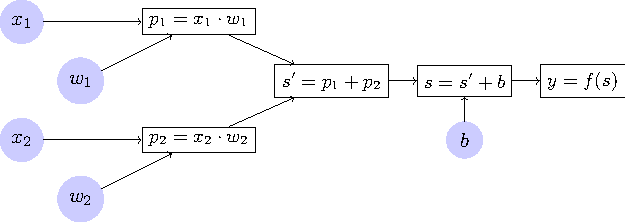
\includegraphics{computational-graph}
	\caption[Ejemplo de grafo computacional.]{Ejemplo de grafo computacional para un perceptrón simple de dos neuronas de entrada y una de salida.}
	\label{fig:computational-graph}
\end{figure}

Una ventaja al representar un modelo como grafo computacional es que ayuda a abstraerse de la formas de las entradas y las salidas, facilitando el trabajo de operaciones en batch. Otra ventaja, todavía mayor, es que, al organizar de entrada a salida (en la figura~\ref{fig:computational-graph} de izquierda a derecha) las operaciones que se necesitan para obtener una salida a partir de una entrada, en los casos donde el objetivo es optimizar la salida permiten fácilmente representar el gradiente al organizarlo del modo contrario (es decir, de las salidas a la entrada o, en el caso de la figura~\ref{fig:computational-graph-derivatives} de derecha a izquierda).

\begin{figure}
	\centering
	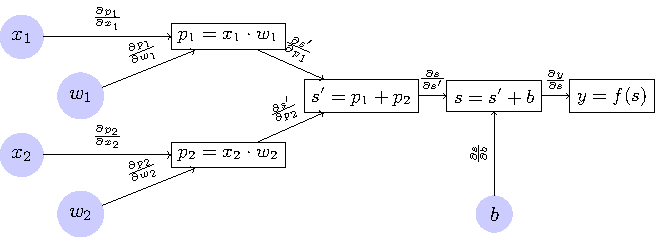
\includegraphics{computational-graph-derivatives}
	\caption[Derivadas parciales sobre un grafo computacional.]{Es fácil representar las derivadas parciales sobre un grafo computacional y, a partir de ahí, obtener el efecto de las variaciones de una variable sobre el resto.}
	\label{fig:computational-graph-derivatives}
\end{figure}

Com regla general, para conocer el gradiente de una variable $a$ con respecto a otra variable $b$, se aplicaría la \textit{regla de la cadena multivariable}, que es equivalente a sumar todos los posibles caminos que van de $a$ a $b$ del grafo, multiplicando las derivadas parciales de cada arista.

\section{\gls{fl}}

La lógica matemática\sidenote{
	\textbf{La lógica nace} en el siglo IV a.C. dentro de la física Aristotélica, que permaneció inalterada hasta la revolución científica (alrededor del siglo XVI. d.C.), momento en que se separó y permaneció como disciplina paralela perteneciente más al campo de la filosofía que de la física y la matemática. Empezó a relacionarse de nuevo con la matemática a principios del siglo XIX y a principios del siglo XX la lógica y la teoría de conjuntos pasaron a convertirse en partes indispensables la una de la otra. Por ello suelen ir de la mano cada vez que se habla de la una y de la otra. La evolución de la teoría de conjuntos (Cantor, finales del siglo XIX, buscar referencia) y su unión con la lógica es una época bastante convulsa dentro de la historia de la matemática.
} (y por extensión la teoría de conjuntos) tiene como misión servir de fundamento del razonamiento matemático. Se basa en la definición precisa y con rigor de un razonamiento evitando cualquier tipo de ambigiüedad y de contradicción. Es por ello que la lógica tradicional no suele servir como fundamento de razonamientos del mundo real.

Los conceptos que se manejan en el mundo real suelen ser vagos, llenos de imprecisiones. Además tienden a ser nombrados cualitativamente, no quantitativamente, y cuando existe una correspondencia, ésta suele estar marcada por la subjetividad de los términos. La lógica difusa se puede considerar como perteneciente al conjunto de lógicas multivaluadas\sidenote{Las lógicas multivaluadas son aquellas donde las premisas pueden tomar más de dos valores.}, donde se trabaja con este tipo de conceptos.

La idea tras este punto de vista es que raramente el ser humano piensa en términos absolutos o completamente definidos. En su lugar, su forma de razonar conlleva una serie de abstracciones que diluyen el caracter de las observaciones que a su vez pueden ser también imprecisas. Ya que en la lógica clasíca es imposible expresar la complejidad que implica la incertidumbre de este proceso de razonamiento, en la \ac{fl} los conceptos de verdad o mentira se relajan, existiendo una transición entre estados no abrupta, sino suave y progresiva.

A lo largo de la sección se describirá el concepto de conjunto difuso, cómo se usan como mecanismo de razonamiento y su utilidad dentro del área de sistemas de control.

\subsection{Ampliando la teoría de conjuntos tradicional}

La teoría de conjuntos difusos nació a mediados del siglo XX de la mano de Lofti A. Zadeh~\cite{lofti1965fuzzy} como solución para la representación de procesos de inferencia conociendo a priori los grados de verdad de las premisas\sidenote{
	La \ac{fl} es uno de esos casos curiosos en la ciencia donde la aplicación nace antes que la propia teoría.
}.A diferencia de los conjuntos tradicionales (\textit{crisp} en la terminología de la \ac{fl}), los conjuntos difusos expresan el grado de pertenencia de un elemento a la categoría representada por el conjunto.

\paragraph{Variables lingüísticas}

El primer concepto importante a entender en la teoría de conjuntos difusos es el de \textbf{variable lingüística}, las cuales sirven de base para toda la teoría porque sus posibles valores son, precisamente, conjuntos difusos. Se define como:

\blockquote{[\ldots] variable whose values are words or sentences in a natural or artificial language [\ldots]}~\cite{zadeh1975concept}

El uso de variables ligüísticas permite representar fenómenos del mundo real como variables cualitativas. Por ejemplo, la variable \textit{velocidad}, puede tomar los valores \textit{atrás rápido}, \textit{atrás lento}, \textit{parado}, \textit{adelante lento} y \textit{adelante rápido}. Es cierto que la variable velocidad a su vez está definida sobre $\mathbb{R}$, y que los conjuntos tienen una definición sobre este dominio, pero la imprecisión que nos dan los términos (conjuntos difusos) se hereda a lo largo de todo el proceso de deducción, de manera similar a como lo hacen los humanos.

\paragraph{Conjuntos difusos}

Una posible definición de conjunto difuso podría ser \textit{dada $X$ una colección de elementos. Se define al \textbf{conjunto difuso} $F$ como un conjunto ordenado de pares de la forma $F = {(x, \mu_F(x)) | x \in X}$, siendo $\mu_F(x) \in [0, 1] \forall x \in X$}. A la función $\mu_F(x)$ se la denomina \textbf{función de pertenencia}, y caracteriza unívocamente a un conjunto difuso del dominio de $X$\sidenote{
	Según Zadeh, la teoría de conjuntos difusos debería servir de ejemplo de lo que él denominó \textit{principio de extensión}~\cite{zadeh1975concept}, esto es, el proceso por el cual generalizar cualquier teoría definida en un dominio discreto hacia su versión continua.
}.

La teoría de conjuntos clásica también define los conjuntos de acuerdo a una función, en este caso denominada \textit{función característica}. Las ecuaciones~\ref{eq:characteristic-function} y~\ref{eq:membership-function} muestran las diferencias entre los valores de $f$ siendo ésta una función característica de la teoría de conjuntos clásica o una función de pertenencia de la teoría de conjuntos difusos respectivamente.

\begin{subequations}
	\begin{equation}
		f(x) = \left\{
			\begin{array}{lcc}
				0 & if & x \notin F \\
				1 & si & x \in F
			\end{array}
		\right.
		\label{eq:characteristic-function}
	\end{equation}
	\begin{equation}
		f(x) = \mu_F(x)
		\label{eq:membership-function}
	\end{equation}
\end{subequations}

Mientras que un conjunto tradicional se basa en si pertenece o no, un conjunto difuso puede\sidenote{
	Puede porque también se puede definir un conjunto \textit{crisp} desde el punto de vista de la lógica difusa.
} tomar todos los valores posibles en el intervalo $[0, 1]$.

\paragraph{Funciones de pertenencia}

Esta función de pertenencia $\mu_F$ puede tomar cualquier forma siempre que estén definidas en el dominio $[0, 1] \subset \mathbb{R}$, pero lo habitual es definirlas como funciones triangulares o trapezoidales. Un ejemplo de estas funciones se ilustra en la figura~\ref{fig:membership-functions}.

\subsection{Razonamiento}

\subsection{Sistemas de inferencia difusa}

Hablar de los tipos de sistemas (Tipos Mandamni y Sugeno diferentes).



-----------------------------------------------------------




\subsection{Teoría de conjuntos difusos}

A diferencia de los conjuntos tradicionales, los conjuntos difusos expresan el grado de pertenencia de un elemento a la categoría representada por el conjunto. La definición podría escribirse de la siguiente manera:

\TODO{Creo que habría que definir antes qué es un dominio}

\begin{definition}
	Sea $X$ una colección de elementos. Se define al \textbf{conjunto difuso} $F$ como un conjunto ordenado de pares de la forma $F = {(x, \mu_F(x)) | x \in X}$, siendo $\mu_F(x) \in [0, 1] \forall x \in X$.
	\label{def:fuzzy-set}
\end{definition}

La función de la definición~\ref{def:fuzzy-set} se denomina \textbf{función de pertenencia}, y caracteriza unívocamente a un conjunto difuso del dominio de $X$.

\TODO{Quizá aquí habría que decir qué es una partición de nu dominio}

\subsection{Operaciones entre conjuntos}

La unión, intersección y el complemento son operaciones básicas en la teoría de conjuntos. \TODO hablar aquí de tnorm, tconorm y complemento, pero someramente. No hay que enrollarse demasiado.

\subsection{Razonamiento}

Al igual que en la lógica tradicional, en la \gls{fl} el razonamiento o inferencia es la manera de extraer conclusiones a partir de premisas en función de un conjunto de reglas.

\sidenote{
	\textbf{La implicación} en lógica se representa como $A \rightarrow B$, donde $A$ es cualquier operación de premisas y $B$ la conclusión que arrojan.
	
	En lógica tradicional, el valor de verdad de una implicación es equivalente al de la expresión $\not A \lor B$. Sin embargo, en lógicas multivaluadas (y por tanto en lógica difusa) esta equivalencia da lugar a razonamientos que se pueden considerar contraintuitivos.
	
	En el caso concreto de la lógica difusa se han propuesto muchas cantidad de equivalencias. Sólo en los trabajos \cite{Kiszka1985} se analizan $72$ alternativas al operador $\not A \lor B$.
	
	El operador más usado no obstante es el definido como $A \land B$ debido a su rendimiento (en la implicación de Mamdani la $T$-norma se implementa como el operador mínimo).
}

Estas reglas se expresan como implicaciones, definidas típicamente en lógica difusa como $A \rightarrow B \equiv A \land B$.

Las dos formas de extraer conclusiones a partir de premisas en \gls{fl} son el \textit{modus ponens} generalizado (del que hablaremos) y el \textit{modus tollens} generalizado, modificaciones sobre los procesos de inferencia \textit{modus ponens} y \textit{modus tollens}\sidenote{
	En realidad se llaman \textit{modus ponendo ponens} (\enquote{la forma que al afirmar, afirma}) y \textit{modus tollendo tollens} (\enquote{la forma que al negar, niega}).
}, dos formas similares de razonamiento (figura~\ref{fig:modus-ponens-and-modus-tollens}). Nosotros centraremos nuestro discurso en la primera.

\begin{figure}
	\missingfigure[figheight=4cm]{Ilustración con las dos formas de razonamiento}
	\caption[\textit{Modus ponendo ponens} vs. \textit{modus tollendo tollens}.]{Formas de razonamiento en lógica tradicional: \textit{modus ponendo ponens} y \textit{modus tollendo tollens}.}
	\label{fig:modus-ponens-and-modus-tollens}
\end{figure}

\newthought{El modus ponens generalizado} es una generalización del modus ponens de la lógica tradicional donde, en lugar de expresas las reglas de forma absoluta, se expresan de forma aproximada. En la figura~\ref{fig:modus-ponens-traditional-vs-generalized} se ilustra las diferencias fundamentales entre ambos modos.

\begin{figure}
	\missingfigure[figheight=4cm]{Ilustración con el modus ponens y el modus ponens generalizado}
	\caption[Diferencias entre \textit{modus ponens} tradicional y generalizado.]{Proceso de razonamiento según el \textit{modus ponens} tradicional frente al \textit{modus ponens} generalizado. En el primero, si la premisa $A$ es cierta, entonces la conclusión $B$ será cierta. En el segundo, dado que la premisa $A$ no es del todo cierta (es $A'$), entonces la conclusión $B$ será cierta sólo en parte ($B'$).}
	\label{fig:modus-ponens-traditional-vs-generalized}
\end{figure}

Para determinar qué grado le asignamos a un consecuente a partir de las premisas parciales y las reglas que dirigen el razonamiento se utiliza un método denominado \textbf{regla composicional de inferencia}.

Una regla $A' \rightarrow B'$ se puede representar como una implicación caracterizada por una función $I(\mu_A(x), \mu_B(y))$ (\cite{Fuller1993}).

\TODO{Explicar mejor porque es terrorífico.}

...

Tengo que hablar también del softmax, el por qué usarlo. También de la entropía cruzada y de por qué usamos este loss sobre el resto.

He visto una cosa curiosa que es el "negative sampling". Podría hablar de ello y usarlo porque haría el entrenamiento mucho más rápido. Por lo que me ha parecido ver, se usa en lugar de la capa softmax y de lo que va es transformar la capa softmax (que es coñazo de calcular) en una capa de k+1 clasificadores binarios, donde hay 1 correcto y k incorrectos. Se usa en clasificación.

En \cite{Ma2004} hay un capítulo de razonamiento que parece que está guay. Revisarlo un poco a fondo a ver si merece la pena tirar or ahí.

\subsection{\gls{fis}}

Los \glspl{fis} (o \glspl{fcs}) son el caso de éxito de la lógica difusa que más resultados ha cosechado tanto a nivel académico como a nivel industrial. Se trata sistemas que utilizan el razonamiento difuso para inferir una respuesta a partir de un conjunto de entradas.

\begin{figure}
	\missingfigure[figheight=4cm]{Ilustración general de un controlador difuso}
	\caption[Diagrama general de un \gls{fis}.]{Diagrama del esquema general de un \gls{fis}.}
	\label{fig:fis-general-schema}
\end{figure}

Habitualmente son descritos como un componente dividido en tres bloques conceptuales:

\begin{itemize}
	\item \textbf{Fuzzificación}. Traducir los valores de entrada en crudo del dominio sobre el que está definida cada variable lingüística a sus respectivos grados de pertenencia a conjuntos difusos a través de sus funciones de pertenencia. \TODO Ojo, algunos controladores toman como valores de entrada conjuntos difusos según \cite{Ma2004}. Habrá que buscar sobre ello.
	\item \textbf{Inferencia}. Realiza todo el proceso de razonamiento difuso a partir del conjunto de reglas qeu dan significado a este controlador difuso.
	\item \textbf{Defuzzificación}. Traduce los conjunto difuso resultado del proceso de inferencia a valores del los dominios sobre los que están definidos dichos conjuntos difusos. \TODO En un sugeno, la salida es una función directamente así que se podría especificar que en un tipo Sugeno,se puede ver como que la salida son sólo singletones, manteniendo la generalización del proceso de funcionamiento de un \gls{fis}.
\end{itemize}

Esta división se ilustra en la figura~\ref{fig:fis-general-schema}.

\newthought{Hay varios tipos diferentes de \gls{fis}}, aunque tienden a seguir el esquema básico de un controlador difuso típico (figura~\ref{fig:fis-general-schema}).

\paragraph{Sistemas de tipo Mandamni}

Son la primera aproximación de \gls{fis} propuestos

\paragraph{Sistemas de tipo Takagi-Sugeno}

...

Hablar someramente de los tres tipos clásicos que se usan, e indicar que al final los más usados son el Mandamni y el Sugeno. Añadir también quizá una tabla comparativa enter los tres o al menos entre los dos principales:

El consecuente de un \gls{fis} de tipo Mandamni siempre es un conjunto difuso. Por tanto, el proceso de sacar un valor crisp es costoso. Lo bueno, se mantiene significado semántico de las salidas. El consecuente en un Sugeno es un valor, y se puede decir que no necesita proceso de defuzzificación. Si embargo, la respuesta pierde significado semántico si la suma de la fuerza de salida no es 1 (no entiendo qué quiero decir con esto).


------------------------------------------


\section{El paradigma de los Agentes Inteligentes}
\label{ch:ci:s:agent-concept}

En la figura~\ref{fig:different-povs-ai} se mostraban los cuatro objetivos perseguidos por la \gls{ai}. En uno de ellos en particular se la entiende como el estudio del conseguir que entidades (e.g. sistemas, software, \ldots) actúen de la manera más inteligente posible. El concepto de \textbf{agente} pertenece a todo el área de la computación, y no únicamente a la \gls{ai}.

Es difícil encontrar un consenso en la definición de agente, y más todavía cuando entra en juego el adjetivo \textit{inteligente}. Sin embargo, sí existen una serie de características que coínciden dentro de la literatura que exponemos a continuación (ver Figura~\ref{fig:agent-properties}):

\begin{itemize}
	\item Operan siempre en un \textbf{entorno}, ya sea éste físico (e.g. una red de carreteras para un vehículo autónomo) o virtual (e.g. un cliente de correo electrónico para un clasificador de spam).
	\item Tienen la capacidad de \textbf{percibir} el entorno por medio de \textit{sensores} y de \textbf{actuar} sobre él por medio de \textit{actuadores}.
	\item Son \textbf{autónomos} en el sentido de que pueden actuar sin intervención externa (e.g. humana u otros agentes) teniendo control sobre su estado interno y su comportamiento. Algunos autores les presuponen una autonomía absoluta mientras que otros hablan de que sólo es necesaria cierta autonomía parcial.
	\item Tienen \textbf{objetivos} a cumplir, actuando para ello sobre el entorno de la manera que les indique su comportamiento.
	\item Pueden ser \textbf{sociales}, es decir, tienen la capacidad de comunicarse con otras entidades (e.g. otros agentes) para llevar a cabo sus objetivos.
\end{itemize}

Nosotros hablaremos de estas entidades desde el punto de vista de la \gls{ai}, y las denominaremos indistintamente \textit{agentes}, \textit{agentes inteligentes} o \textit{agentes racionales}\sidenote{
	El término preferido en esta tésis es precisamente este último, \textbf{agentes racionales}, dado que captura la esencia de lo que es un comportamiento inteligente. El problema de este punto de vista es que, como bromean en~\cite{russell2003artificial}, hasta un elemento tan rudimentario como un termostato puede ser considerado un elemento inteligente, ya que realiza siempre la mejor acción para cumplir sus objetivos por muy simples que puedan parecer. Pero, ¿qué hace a un agente inteligente? Según algunos autores, el hecho de que posea unos objetivos y autonomía suficiente para cumplirlos ya denota inteligencia (e.g. en~\cite{russell2003artificial}). Según otros, es necesario que el comportamiento sea flexible, esto es, que sea reactivo (reacciona ante el entorno que percibe), proactivo (iniciativa para tratar de cumplir sus objetivos) y social (capaz de interactuar con otros agentes para cumplir sus objetivos) (e.g.~\cite{Wooldridge1995}). Y otros directamente exigen, además, un comportamiento racional a la hora de cumplir los objetivos para calificarlo de inteligente (e.g.~\cite{shoham1993agent}). Como dijimos anteriormente, dónde está el límite entre qué es y que no es un inteligente cae dentro de los dominios de la filosofía.
}. Por tanto usaremos la siguiente definición:

\blockquote{Un agente es una entidad física o virtual que realiza una acción\sidenote{
		En \cite{russell2003artificial} se define como \textit{\enquote{\ldots just something that acts}} alegando que la palabra \textit{agent} proviene del latín \textit{agere}. Para clarificar esto, \textit{agere} es la forma verbal para \textit{hacer}, pero imprime un significado de movimiento/actividad diferente que no tiene mucho que ver con \textit{hacer} como forma verbal para \textit{crear} o \textit{dar forma} (de lo que se ocupa el verbo \textit{facere}). Por ello, el verbo \textit{actuar} es un verbo que se relaciona con \textit{agere} y de ahí la definición.
	} de manera total o parcialmente autónoma dada una secuencia de percepciones del entorno en el que se ubica.}

\begin{figure}[t]
	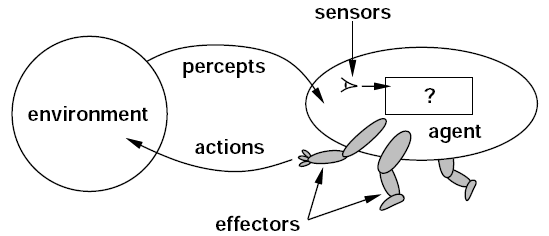
\includegraphics{agent-properties}
	\caption[Esquema de agente y sus propiedades.]{Esquema de un agente y sus propiedades. Aunque no existe una definición comúnmente aceptada de agente, sí que existe una serie de propiedades que los que los identifican. Es autónomo, opera realiza acciones sobre un entorno dependiendo de las percepciones que le llegan de éste y tiene la capacidad de comunicarse con el resto de elementos, incluídos otros agentes.\TODO{CAMBIAR LA IMAGEN Y VER CÓMO SE PUEDE INCLUIR EL CONCEPTO DE COLABORACIÓN}}
	\label{fig:agent-properties}
\end{figure}

Según ésta, un agente es considerado \textbf{agente inteligente} cuando éste realiza la mejor acción posible (según un criterio de medida). En este contexto, \textit{la mejor acción posible} se refiere en términos de objetivos a cumplir y comprensión del entorno en el que se desarrolla la acción, que puede ser o no correcta.

Las nociones de agentes inteligentes y la de \gls{ci} van de la mano. Esto es debido a que su definición funciona a la perfección para las técnicas de la \gls{ci}, esto es, agentes autónomos que perciben el entorno (problema) y actuan de la mejor manera posible sobre él (resuelven) de acuerdo a su conocimento del medio y su estado interno (en base a algoritmos como \gls{ann}, \gls{fl}, \ldots). Por ello desde mediados de los años 1990 el concepto de agente inteligente ha ganado tanta popularidad\sidenote{Tanto es así que en algunos trabajos se define el objetivo de la \gls{ai} como la implementación de la función agente, esto es, la función que realiza la correspondiencia de una percepción a una acción, para un problema dado.}.

\subsection{Tipos de entorno}

La tupla \textit{(entorno, agente)} es esencialmente una metáfora para referirse a la tupla \textit{(problema, solución)} por lo que existen casi tantos entornos diferentes como problemas.

Afortunadamente es posible caracterizar los entornos de acuerdo a un conjunto de propiedades o dimensiones. Este conjunto es usado por la totalidad de la literatura a la hora de caracterizar entornos:

\begin{itemize}
	\item \textbf{Observable}. Un entorno es \textbf{totalmente observable} cuando el agente es capaz de captar toda la información relevante para la toma de una decisión y no necesita mantener ningún modelo interno del entorno, \textbf{parcialmente observable} cuando la información obtenida es incompleta o tiene ruido y \textbf{no observable} cuando el agente no posee sensores.
	\item \textbf{Multiagente o. monoagente}. Un entorno es \textbf{multiagente} cuando requiere de múltiples agentes interactuando para llegar a una solución mientras que es \textbf{monoagente} cuando sólo requiere de uno para ello.
	\item \textbf{Determinista o. no determinista}. Si el estado del entorno actual depende totalmente del estado anterior, se dice que el entorno es \textbf{determinista}. Si no es así, se considera \textbf{no determinista} o \textbf{estocástico}\sidenote{
		En general, los entornos del mundo real tienden a ser tan complejos que es imposible para un agente abarcar todos los aspectos medibles de éste. Por lo tanto, sea o no la naturaleza del entorno determinista, en general se suele suponer éste como no determinista.
	}.
	\item \textbf{Episódico o. secuencial}. Un entorno en el que las acciones se dividen atómicamente donde cada una de ellas conlleva un ciclo de (percepción, decisión, acción) y sin relación una con otra se denomina episódico. Si en lugar de ello la acción del agente puede afectar a las decisiones futuras se dice que el entorno es \textbf{no episódico} o \textbf{secuencial}.
	\item \textbf{Estático o. dinámico}. Si durante la toma de decisioń en entorno no cambia, se dice que el entorno es \textbf{estático}. En caso contrario, se dice que es \textbf{dinámico}.
	\item \textbf{Discreto o. continuo}. Esta dimensión en realidad se divide en cuatro, estado del entorno, tiempo en el entorno, percepciones y acciones. La dimensión es \textbf{discreta} cuando ésta se divide en una partición discretizada, y \textbf{continua} cuando no. Por ejemplo, en el Juego de la Vida de Conway, si se modela en un sistema multiagente, tanto el estado (i.e. tablero) como el tiempo (i.e. turnos) como las percepciones y acciones están discretizadas. Sin embargo, en un entorno de conducción automática se puede determinar que las cuatro dimensiones son continuas.
	\item \textbf{Conocido o. desconocido}. Un entorno es \textbf{conocido} cuando es posible determinar cuál va a ser el resultado de una acción. Si por el contrario no es posible, entonces se dice que es \textbf{desconocido}\sidenote{
		Que el conocimiento del entorno no sea total es un factor clave que diferencia la racionalidad de la omnisciencia. La omnisciencia significa conocer el resultado de toda acción antes de realizarla y por tanto implica el conocimiento de absolutamente todos los detalles del entorno. La racionalidad existe dentro de un contexto de conocimiento limitado.
	}.
\end{itemize}

\subsection{Arquitecturas}

Existe una serie de arquitecturas básicas o tipos de agentes que dependen principalmente de cómo perciben el entorno y de qué forma se comportan aunque, dependiendo de los autores, las nomenclaturas, tipologías y esquemas pueden variar. Por ello, hemos decidido ofrecer una abstracción donde poner de manifiesto las partes comunes y no comunes entre arquitecturas.

\begin{figure}
	\missingfigure[figheight=3.5cm]{Arquitectura básica de un agente}
	\caption[Arquitectura básica de un agente.]{Arquitectura básica de un agente. Aunque existen múltiples arquitecturas diferentes, todas se basan en la misma estructura. El agente percibe el entorno, lo interpreta y toma la decisión de cómo actuar sobre él.}
	\label{fig:agent-basic-architecture}
\end{figure}

La figura~\ref{fig:agent-basic-architecture} muestra el esquema de las partes principales de un agente. En general, todo arquitectura de agente inteligente está cortada por el mismo patrón y obedece al siguiente funcionamiento:

\begin{enumerate}
	\item El agente, a través de sus \textbf{sensores}, percibe el entorno en el que éste se mueve.
	\item De acuerdo a cómo recordamos el entorno (llamémoslo \textbf{modelo del entorno}), el agente genera una \textbf{interpretación del entorno} tal y como supone el agente que es. Esto es, percibe el entorno y, de acuerdo a sus sensaciones, lo entiende de una determinada forma.
	\item Esta interpretación del entorno es pasada a un proceso de \textbf{inferencia} el cual, en función la implementación para la consecución de sus objetivos, generará una serie de acciones a realizar sobre el entorno.
	\item Estas acciones serán ejecutadas sobre el entorno a través de una serie de \textbf{actuadores}, provocando probablemente una modificación en éste que será percibida de nuevo en momentos sucesivos.
\end{enumerate}

La primera diferencia clave surge en la manera que se ofrece al bloque de inferencia la interpretación del entorno y genera la primera clasificación (figura~\ref{fig:memory-vs-amnesia-in-agents}):

\begin{figure}
	\missingfigure[figheight=3.5cm]{Arquitectura básica de un agente}
	\caption[Diferencias entre un agente sin y con modelo de entorno.]{Ilustración de la diferencia entre un agente sin modelo de entorno y uno con modelo de entorno. Cada acción realizada por el agente con modelo de entorno tiene en cuenta el estado del entorno en momentos pasados. El agente sin modelo de entorno actúa tal y como interpreta el entorno en cada momento, como si sufriese de amnesia.}
	\label{fig:memory-vs-amnesia-in-agents}
\end{figure}

\begin{itemize}
	\item \textbf{Sin modelo de entorno}. Si el agente ofrece su interpretación del entorno directamente, sin hacer uso de información histórica sobre el entorno que se ha movido. Otras formas de denominar a estos agentes es como \textit{agentes reactivos} o \textit{simple-reflex agents} (\cite{russell2003artificial}). Sin embargo, los términos \textit{reactivo} o \textit{reflex} para algunos autores se refieren a la forma de inducción de acciones a partir de percepciones, y por ello preferimos la denominación \textit{sin modelo de entorno}.
	\item \textbf{Con modelo de entorno}. El agente genera su interpretación más detallada del entorno a partir de las percepciones que llegan desde los sensores y de el histórico del entorno que mantiene. Otras formas de llamarlo es \textit{agentes con estado} o \textit{Model-based}, pero lo hemos denominado de esta manera para diferenciar que el modelo que se mantiene en este punto pertenece únicamente al entorno.
\end{itemize}

\begin{figure}
	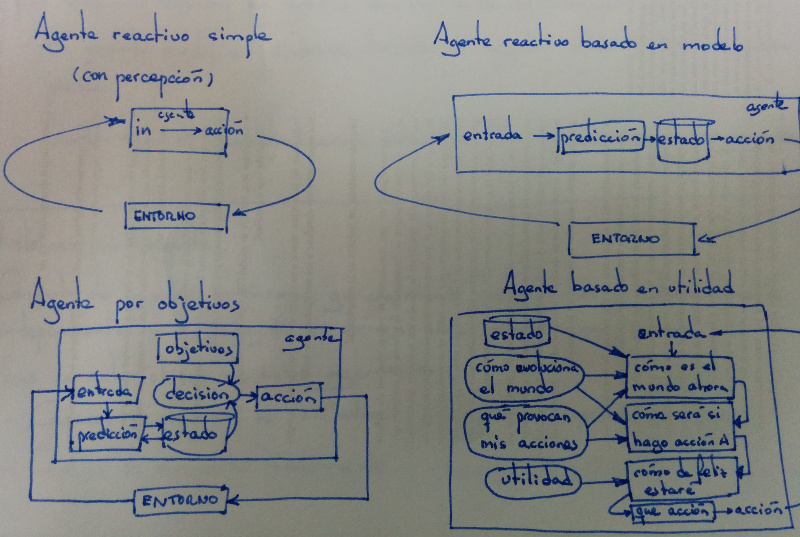
\includegraphics{agent-types}
	\caption[Arquitecturas de agente según su comportamiento.]{Distintas arquitecturas de agentes en función del comportamiento. Dependiendo de las acciones a realizar, se identifican tres tipos, los reactivos que aplican una acción sin proceso deductivo y los basados en modelo y utilidad (en algunos contextos denominados deliberativos) que basan su comportamiento en alguna forma de deducción.}
	\label{fig:agent-types}
\end{figure}

La siguiente clasificación viene motivada por la forma de deducir el conjunto de acciones a ser aplicadas por parte de los sensores. En este sentido podemos identificar tres tipos distintos de agentes (figura\ref{fig:agent-types}):

\begin{itemize}
	\item \textbf{Reactivos}. Son aquellos donde el uso de un proceso de razonamiento explícito es demasiado costoso para producir una conducta en un tiempo aceptable. Se suelen implementar como correspondencias (percepción $\rightarrow$ acción) sin ningún razonamiento adicional.
	\item \textbf{Basados en objetivos}. Plantean una deducción de forma que determinan cuál sería el estado del entorno tres aplicar varias o todas las acciones que puede realizar. En base a los resultados, selecciona la acción que se corresponde con sus propios objetivos.
	\item \textbf{Basados en utilidad}. Éstos plantean una deducción similar a los basados en objetivos con la diferencia de que, mientras los primeros sólo diferencian entre entorno objetivo o no objetivo, éstos asignan un valor (i.e. \textit{utilidad}) a cada uno de los escenarios de entorno posibles para seleccionar el mejor (e.g. el que mayor utilidad tiene).
\end{itemize}

En la literatura se describen muchos tipos de agente, como por ejemplo los agentes BDI (Believe-Desire-Intention) o los agentes lógicos (i.e. el entorno se representa con reglas lógicas y se infiere mediante métodos como por ejemplo deducción lógica o prueba de teoremas). Sin embargo, éstos pueden definirse en los términos aquí expuestos (figuras~\ref{fig:agent-basic-architecture}, \ref{fig:memory-vs-amnesia-in-agents} y \ref{fig:agent-types}). 

\subsection{\gls{mas}}

Son aquellos sistemas compuestos de dos o más agentes que interactúan de alguna manera para llegar a una solución.

Cuando los agentes son inteligentes y el problema cae dentro del dominio de la \gls{ai}, el ámbito de estudio es el de la \gls{dai}, la rama dedicada a la resolución de problemas mediante procesamiento descentralizado.

Desde el punto de vista de la ingeniería de sistemas, y a pesar del aumento de complejidad, los \gls{mas}, al ser sistemas inherentemente descentralizados, ofrecen múltiples ventajas frente a los sistemas centralizados tradicionales:

\begin{itemize}
	\item Los sistemas son más robustos y fiables frente a fallos, ya que los agentes son autónomos e independientes del resto.
	\item La modificación del sistema se puede realizar sobre la marcha, agente a agente sin necesidad de parar el sistema al completo.
	\item Su diseño fuerza a desacoplar las dependencias entre agentes.
	\item Son inherentemente paralelizables y por tanto pueden llegar a ser más eficientes que sus homólogos centralizados. Este punto es quizá el más controvertido, ya que esta ganancia en eficiencia se puede perder rápidamente en función de la cantidad de comunicación existente entre agentes.
	\item Debido al nivel de complejidad alcanzado en los sistemas existentes en la actualidad, la computación se distribuye a través de múltiples sistemas, normalmente heterogéneos. La tendencia además es a la alza. La definición de los \gls{mas} hace natural su implementación en este tipo de arquitecturas.
\end{itemize}

Desde el punto de vista de la \gls{ai} podemos añadirles la ventaja de que permiten el estudio de conductas complejas de poblaciones a partir del comportamiento de sus elementos básicos, facilitando el estudio de modelosy de teorías sobre éstos.

\newthought{La comunicación entre agentes}, se trata de una característica clave en un \gls{mas}, ya que para denominarse de esta manera dos o más agentes deben interactuar (i.e. comunicarse) entre si. Esta interacción puede implementarse de diversas maneras\sidenote{Las formas clásicas de comunicación son el de paso de mensajes, los sistemas de pizarra y la estigmergia. Para los dos primeros existen dos propuestas para estándar de lenguaje de comunicación, \gls{kqml} (\cite{Finin1994}) y \gls{acl} (\cite{Poslad2007}). La tercera forma de comunicación suele ser muy dependiente del problema y no se apoya en lenguajes estándares. Se trata de una forma de comunicación basada en la modificación del entorno, como la efectuada por las hormigas en la búsqueda de alimento, donde éstas dejan rastros de feromonas modificando el entorno para modificar el comportamiento del resto de la colonia.} y siempre toman una o las dos formas siguientes (figura~\ref{fig:communication-between-agents-in-mass}):

\begin{itemize}
	\item \textbf{Cooperación}. Los agentes intercambian información entre sí para llegar a una solución. Esta solución puede ser fragmentada (i.e. cada agente posee parte de la solución y se comunican para ir avanzando de forma común hacia la solución global) o poseerla uno o varios agentes que hacen uso de más agentes para ir avanzando la solución.
	\item \textbf{Competición}. Los agentes compiten dentro de un entorno, generalmente mediante la adquisición de recursos limitados. Un ejemplo de este tipo de sistemas multiagente puede ser aquellos sistemas de vida artificial.
\end{itemize}

\begin{figure}
	\missingfigure[figheight=3.5cm]{Una ilustración de algún entorno de vida artificial donde los agentes compiten y uno de algo donde cooperen}
	\caption[Diferencias entre colaboración y competitividad de agentes.]{La comunicación entre agentes puede ser de dos tipos: \textit{colaborativa}, donde los agentes tratan de llegar a una solución intercambiándose información y \textit{competitiva}, donde los agentes compiten unos contra otros en un entorno.}
	\label{fig:communication-between-agents-in-mass}
\end{figure}
